\documentclass[10pt,twocolumn]{article}

\usepackage[utf8]{inputenc}
\usepackage[T1]{fontenc}
\usepackage[margin=0.72in,columnsep=0.24in]{geometry}
\usepackage{microtype}
\usepackage{amsmath,amssymb,amsthm}
\usepackage{graphicx}
\usepackage{booktabs}
\usepackage{multirow}
\usepackage{array}
\usepackage{natbib}
\usepackage{xcolor}
\usepackage{algorithm}
\usepackage{algpseudocode}
\usepackage{caption}
\usepackage{subcaption}
\usepackage{hyperref}

\hypersetup{
  colorlinks=true,
  linkcolor=blue!60!black,
  citecolor=blue!60!black,
  urlcolor=blue!60!black
}

\captionsetup{font=small,labelfont=bf}
\setlength{\tabcolsep}{4.2pt}

\newtheorem{proposition}{Proposition}
\newtheorem{remark}{Remark}

\title{\textbf{Bayesian Generalized Nonlinear Models Offer Basis-Free SINDy with Calibrated Model Uncertainty}}

\author{
  \textbf{Aliaksandr Hubin}$^{1}$ \\
  $^{1}$Faculty of Chemistry, Biotechnology and Food Science, NMBU; \\
  Faculty of Health, Welfare and Organisation, HiOF; \\
  Department of Mathematics, University of Oslo, Norway \\
  \texttt{aliaksandr.hubin@nmbu.no}
}

\date{}

\begin{document}
\maketitle

\begin{abstract}
Sparse Identification of Nonlinear Dynamics (SINDy) has become a foundational paradigm for discovering governing differential equations from time-series data. However, classical SINDy and bagging/Bayesian SINDy variants rely on a fixed, predefined candidate library: omitting the true nonlinearity causes structural misspecification, whereas stuffing an overcomplete dictionary triggers severe multicollinearity and combinatorial blowup. Conversely, heuristic/evolutionary symbolic regression avoids predefined bases but typically lacks calibrated Bayesian uncertainty quantification and exhibits high run-to-run instability. Building upon our preliminary three-system study \citep{hubin2025bgnlm} and the \texttt{FBMS} package \citep{lachmann2025fbms}, we develop a systematically tuned, identifiability-preserving \textbf{Bayesian Generalized Nonlinear Model (BGNLM)} framework for basis-free dynamical system discovery. Our tuned BGNLM combines unknown-variance unit-information/Jeffreys-BIC marginal likelihoods, complexity-penalized model priors ($r=N^{-1}$), radian-scaled physical operator sets, disabled unidentifiable projection steps ($p_{\text{proj}}=0$), a low-dimensional collinearity guard, and parallel Genetically Modified Mode Jumping MCMC (GMJMCMC) with median probability selection and post-hoc $L_2$-energy pruning. Across a large-scale benchmark of \textbf{109,192 synthetic runs} spanning 12 dynamical systems (additive derivative noise; polynomial, transcendental/rational, and 5D coupled Lorenz-96) and \textbf{2,600 quasi-empirical runs} across 5 canonical literature-parameterized ODE benchmarks with noisy state observations and numerical differentiation, evaluated with hierarchical Linear Mixed-Effects Models (LMMs) incorporating system-by-method random interactions and Dunnett multiplicity adjustment, tuned BGNLM achieves the lowest false discovery rate ($\text{FDR}=0.102$) and overall structure recovery $\text{F1}=0.847$---statistically indistinguishable from an oracle-basis Bayesian upper bound ($\text{F1}=0.859, p_{\text{adj}}=1.000$) while significantly outperforming CV-BIC-tuned STLSQ ($\text{F1}=0.600$ poly, $0.698$ oracle), 80-replicate bagged STLSQ ($\text{F1}=0.495$--$0.560$), explicit rational STLSQ ($\text{F1}=0.425$), static-pool Pareto/MDL symbolic regression ($\text{F1}=0.538$--$0.554$), and the untuned IWSM baseline ($\text{F1}=0.562$). On 5D Lorenz-96, tuned BGNLM ranks \#1 across all 13 methods ($\text{F1}=0.983$, exact recovery $80.6\%$), and on the quasi-empirical noisy-state suite it ranks \#1 among all basis-free methods ($\text{F1}=0.624$, $R^2_{\text{traj}}=0.764$, $92.5\%$ empirical 95\% coverage) at roughly half the equation complexity of oracle baselines.
\end{abstract}

% ==============================================================================
\section{Introduction}
% ==============================================================================

Inferring parsimonious governing ordinary differential equations (ODEs) $\dot{\boldsymbol{x}}(t) = \boldsymbol{f}(\boldsymbol{x}(t))$ directly from noisy measurements is central to modern scientific machine learning. Sparse Identification of Nonlinear Dynamics (SINDy) \citep{brunton2016discovering} frames equation discovery as sparse linear regression $\dot{\boldsymbol{x}} \approx \boldsymbol{\Theta}(\boldsymbol{x})\boldsymbol{\Xi}$ over a predefined dictionary $\boldsymbol{\Theta}(\boldsymbol{x})$ via sequentially thresholded least squares (STLSQ). Subsequent advances introduced implicit/rational libraries (SINDy-PI) \citep{kaheman2020sindy}, weak formulations \citep{messenger2021weak}, bagging ensembles (Ensemble-SINDy) \citep{fasel2022ensemble}, and Bayesian sparsifying priors (UQ-SINDy) \citep{hirsh2022sparsifying} to quantify parameter uncertainty.

Despite these advances, dictionary-based methods face a fundamental \emph{library dilemma}:
\begin{enumerate}
  \item \textbf{Misspecification}: Standard degree-$d$ polynomial dictionaries cannot represent trigonometric, fractional, exponential, or Michaelis--Menten/Hill kinetics without prior domain knowledge, causing complete failure in exact structure recovery.
  \item \textbf{Multicollinearity in overcomplete dictionaries}: Attempting to cover all plausible nonlinearities in one static matrix $\boldsymbol{\Theta}(\boldsymbol{x})$ produces dozens or hundreds of strongly correlated columns, inflating false discovery rates (FDR), destabilizing sparse regression, and breaking $p > n$ estimation on scarce empirical data.
\end{enumerate}

Symbolic Regression (SR) frameworks such as Eureqa \citep{schmidt2009distilling}, PySR \citep{cranmer2023interpretable}, and PyOperon \citep{burlacu2020operon} circumvent fixed dictionaries via evolutionary expression-tree search. However, genetic programming returns deterministic Pareto fronts rather than posterior distributions over equation space: it provides neither calibrated posterior inclusion probabilities (PIPs) nor Bayesian predictive credible intervals, and suffers substantial seed-to-seed structural instability \citep{lacava2021contemporary}.

In our preliminary workshop study \citep{hubin2025bgnlm}, we proposed applying Bayesian Generalized Nonlinear Models (BGNLMs) \citep{hubin2021flexible} as a basis-free Bayesian alternative to SINDy, evaluating an untuned prototype on three 3D ODEs. While promising at low noise, that prototype relied on fixed dispersion $\sigma^2=1$, degree-scaled trigonometry (\texttt{sin\_deg}/\texttt{cos\_deg}), unpruned nested projections, small populations, and lacked comparisons against predefined-basis Bayesian models, modern SINDy variants, SR baselines, and real-world data.

In this work, we resolve these limitations and deliver a comprehensive ICML-scale methodology and empirical evaluation using the \texttt{FBMS} engine \citep{lachmann2025fbms}. Our main contributions are:
\begin{itemize}
  \item \textbf{Principled, Identifiability-Preserving BGNLM-SINDy}: We show why naive GMJMCMC hyperparameter defaults fail on dynamical systems (projection nesting, degree-scaled trig, and low-dimensional collinearity check underflow) and establish a systematically tuned configuration combining unknown-variance BIC/unit-information likelihoods, $r=N^{-1}$ complexity penalties, radian physical transforms, $p_{\text{proj}}=0$, and $L_2$-energy pruning.
  \item \textbf{Expanded 12-System Synthetic Benchmark (109,192 Runs)}: We evaluate 13 methods across 7 polynomial ODEs (Group A), 4 non-polynomial trigonometric/rational ODEs (Group B), and 5D coupled Lorenz-96 (Group C) across 5 sample sizes $N \in [100, 2500]$ and 7 derivative noise levels $\sigma \in [0.001, 1.0]$, testing selection consistency, exact recovery, Nogueira stability, PIP calibration, and ODE rollout fidelity, including held-out validation on the 9 systems excluded from tuning.
  \item \textbf{5 Quasi-Empirical Noisy-State Benchmarks (2,600 Runs)}: On 5 canonical literature-parameterized physical and biological ODE systems with additive state observation noise, rolling temporal cross-validation, and Savitzky--Golay vs.\ TV-regularized numerical differentiation, we evaluate ecology, microcosm, lab mechanics, hydraulic, and biochemical dynamics.
  \item \textbf{Rigorous Mixed-Effects Statistical Inference}: Rather than informal table-gazing, we evaluate all benchmark outcomes using hierarchical Linear Mixed-Effects Models (LMMs) with random intercepts and \emph{system/dataset-by-method random interactions}, Dunnett multiplicity adjustment, regime moderation tests, binomial exact-recovery GLMMs, and complete ICC variance decompositions.
  \item \textbf{Reproducible Open Benchmark Suite}: All code, symbolic AST equivalence checkers, tuning logs, and checkpoints are reproducibly packaged on the \texttt{ICML} branch of \url{https://github.com/aliaksah/BGNLM-for-SINDy}.
\end{itemize}

% ==============================================================================
\section{Bayesian Generalized Nonlinear Models for Dynamical Systems}
% ==============================================================================

\subsection{Hierarchical State-Space Formulation}

Consider an $m$-dimensional autonomous (or input-driven) dynamical system
\begin{equation}
  \dot{\boldsymbol{x}}(t) = \boldsymbol{f}(\boldsymbol{x}(t), \boldsymbol{u}(t)), \qquad \boldsymbol{x}(t) \in \mathbb{R}^m,
\end{equation}
observed at $N$ time points $\{t_i\}_{i=1}^N$ yielding state observations $\boldsymbol{X} \in \mathbb{R}^{N \times m}$ and numerically estimated or noisy derivative observations $Y_{ji} = \dot{x}_j(t_i) + \varepsilon_{ji}$ for each component $j \in \{1,\dots,m\}$, with $\varepsilon_{ji} \stackrel{\text{iid}}{\sim} \mathcal{N}(0, \sigma_j^2)$. Note that in Experiment~1 states $\boldsymbol{X}$ are observed cleanly while Gaussian noise enters $\boldsymbol{Y}$ directly (isolating derivative SNR scaling without errors-in-variables attenuation), whereas Experiment~2 injects state measurement noise prior to numerical differentiation.

Rather than fixing a static library $\boldsymbol{\Theta}(\boldsymbol{x})$, BGNLM models each component $j$ conditionally on a dynamically evolved finite feature population $\mathcal{F}_j = \{g_1(\boldsymbol{x}), \dots, g_q(\boldsymbol{x})\} \subset \mathcal{G}_D$ of algebraic and transcendental expression trees of depth at most $D$:
\begin{equation}
  Y_{ji} \mid \boldsymbol{\gamma}_j, \boldsymbol{\beta}_j, \sigma_j^2 \sim \mathcal{N}\!\left(\beta_{j0} + \sum_{k=1}^{q} \gamma_{jk}\beta_{jk}g_k(\boldsymbol{x}_i), \; \sigma_j^2\right),
\end{equation}
where $\gamma_{jk} \in \{0,1\}$ are binary inclusion indicators and $\boldsymbol{\beta}_{j,\boldsymbol{\gamma}_j}$ are the active regression coefficients under configuration $\boldsymbol{\gamma}_j$.

\subsection{Complexity-Penalized Model \& Parameter Priors}

Following \citet{hubin2021flexible,lachmann2025fbms}, each nonlinear feature $g_k \in \mathcal{G}_D$ carries an operational tree complexity $c(g_k) \ge 1$ (e.g., $c(x_l)=1$, $c(x_l x_r)=2$, and deeper compositions accumulate operator costs). Conditional on the finite feature population $\mathcal{F}_j^{(p)} \subset \mathcal{G}_D$ explored at generation $p$, we assign a complexity-penalized hierarchical Bernoulli model prior:
\begin{equation}
  p(\boldsymbol{\gamma}_j \mid \mathcal{F}_j^{(p)}) \propto \prod_{k=1}^{q} r^{c(g_k)\,\gamma_{jk}}, \qquad r = N^{-1}.
\end{equation}
Taking logarithms, adding a feature of complexity $c(g_k)$ incurs an explicit log-prior penalty $c(g_k)\log r = -c(g_k)\log N$. Within each GMJMCMC generation, model probabilities are normalized over $\mathcal{F}_j^{(p)}$ and aggregated across populations weighted by marginal likelihood mass \citep{hubin2021flexible}.

For the regression parameters $(\beta_{j0}, \boldsymbol{\beta}_{j,\boldsymbol{\gamma}_j}, \sigma_j^2)$ given model $\boldsymbol{\gamma}_j$ of active dimension $p_{\gamma} = |\boldsymbol{\gamma}_j|$, we compare four conjugate/analytical marginal likelihood formulations inside \texttt{FBMS}:
\begin{enumerate}
  \item \textbf{Unit-Information / Jeffreys-BIC with Unknown Variance ($\sigma_j^2$ free)}: Approximates the marginal likelihood via the Schwarz/BIC Laplace expansion under a proper unit-information parameter prior \citep{kass1995reference} paired with the Jeffreys scale prior $p(\sigma_j^2) \propto \sigma_j^{-2}$, yielding $\log p(\boldsymbol{y}_j \mid \boldsymbol{\gamma}_j) = -\frac{N}{2}\log(\text{RSS}_{\boldsymbol{\gamma}_j}/N) - \frac{p_{\gamma}+1}{2}\log N + O(1)$ (including the intercept degree of freedom and avoiding improper-prior normalizing ambiguities). Combined with Eq.~(3), adding a term of complexity $c(g_k)$ pays total log penalty $(c(g_k) + \tfrac{1}{2})\log N$. Crucially, leaving $\sigma_j^2$ unknown adapts automatically across SNR regimes spanning $\sigma \in [10^{-3}, 1.0]$, in contrast to our earlier untuned IWSM baseline which fixed $\sigma_j^2 = 1.0$.
  \item \textbf{Zellner's $g$-Prior} \citep{zellner1986assessing}: $\boldsymbol{\beta}_{j,\boldsymbol{\gamma}_j} \mid \sigma_j^2, \boldsymbol{\gamma}_j \sim \mathcal{N}(\mathbf{0}, g\,\sigma_j^2 (\boldsymbol{G}_{\boldsymbol{\gamma}_j}^\top \boldsymbol{G}_{\boldsymbol{\gamma}_j})^{-1})$ with $g = \max(N, p^2)$ and unknown $\sigma_j^2$, providing closed-form marginal likelihoods with scale-invariant collinearity shrinkage.
  \item \textbf{Mixtures of $g$-Priors}: Truncated Compound Confluent Hypergeometric (\texttt{robust} tCCH) and \texttt{hyper-g/n} priors \citep{liang2008mixtures}.
\end{enumerate}

\subsection{Identifiability, Low-D Collinearity Fix, and Pruning}

Deploying \texttt{FBMS} successfully on dynamical systems required resolving three structural pitfalls uncovered during systematic calibration:
\begin{enumerate}
  \item \textbf{Disabling Projection Mutations ($p_{\text{proj}} = 0$)}: General GMJMCMC supports linear-combination projection nodes $h(1 + \sum \alpha_l g_l)$. When composed with nonlinear activations (e.g., $\sin(1 + x_1 + x_2^2)$ or $(1 + x_1 + x_2)^3$), projection features break algebraic identifiability, inflate false discoveries, and trigger exponential AST blowup during post-hoc canonicalization. Setting $p_{\text{proj}} = 0$ with pure algebraic/operator search ($p_{\text{inter}} = 0.55$, $p_{\text{mod}} = 0.35$, $p_{\text{new}} = 0.10$, depth $D \le 2$) preserves clean physical structure. As an expressivity trade-off, $p_{\text{proj}}=0$ restricts unary nonlinearities to unit internal scales (e.g., $\sin(x_1)$ or $x_3^2/(1+x_3^2)$ rather than $\sin(\omega x_1)$ for $\omega \neq 1$), which suffices for canonical dimensionless ODEs; non-unit internal frequencies would require re-enabling parameterized projections.
  \item \textbf{Radian-Scaled Physical Operators}: Replacing degree-scaled trigonometry (\texttt{sin\_deg}, \texttt{cos\_deg}) with exact radian and saturation/rational operators (\texttt{sin\_rad}, \texttt{cos\_rad}, \texttt{p2}, \texttt{p3}, \texttt{p05}, \texttt{pm1}, \texttt{exp\_neg}, \texttt{inv\_pos}, \texttt{inv\_sq}, \texttt{hill\_2}, \texttt{sigmoid}) aligns the operator pool with physical units (e.g., pendulum $\sin(x_1)$ and Michaelis--Menten $x_3^2/(1+x_3^2)$).
  \item \textbf{Low-Dimensional Collinearity Guard}: In \texttt{FBMS}, \texttt{check.collinearity} subsamples $n_{\text{col}} = 2 p_0$ rows to test rank deficiency, where $p_0 = m$ is the number of raw inputs. For 2D/3D ODEs ($n_{\text{col}} \in \{4,6\}$), \texttt{lm.fit} encounters $p > n_{\text{col}}$ as soon as $|\mathcal{F}_j| \ge 4$, causing premature population stalls. Increasing the check subsample to $n_{\text{col}} = \min(N, \max(2p_0, 3|\mathcal{F}_j|+15))$ and dropping zero-variance covariates prior to MCMC restores full exploration.
\end{enumerate}

After running $R=6$ parallel GMJMCMC chains ($P=12$ populations, $N_{\text{MCMC}}=500$ iterations per population, $\text{pop.max}=20$), we extract the Median Probability Model (MPM) \citep{barbieri2004optimal} $\{g_k : \widehat{\text{PIP}}_{jk} = \hat{p}(\gamma_{jk} = 1 \mid \boldsymbol{D}) > 0.5\}$ and apply \emph{relative $L_2$-energy pruning}: a selected atom $g_k$ is retained iff
\begin{equation}
  \frac{|\hat{\beta}_{jk}| \, \|g_k(\boldsymbol{X})\|_2}{\|\boldsymbol{y}_j\|_2} \ge \tau_{\text{energy}}, \qquad \tau_{\text{energy}} = 0.025,
\end{equation}
discarding tiny spurious noise terms before refitting OLS on $\hat{\mathcal{S}}_j$. Note that this pruning step acts as a pragmatic finite-sample structural filter after Bayesian selection (and reported PIP Brier scores evaluate unpruned MJMCMC PIPs). For predictive uncertainty, we construct a pragmatic hybrid 95\% predictive interval centered at the post-pruning OLS mean $\hat{\mu}_{\text{OLS}}(\boldsymbol{x}_*)$ with half-width $\sqrt{h_{\text{BMA}}(\boldsymbol{x}_*)^2 + (1.96\,\hat{s}_*)^2}$, combining the unpruned \texttt{FBMS} BMA quantile half-width $h_{\text{BMA}}$ with the post-selection predictive standard error $\hat{s}_* = \hat{\sigma}_j \sqrt{1 + \boldsymbol{g}_*^\top (\boldsymbol{G}^\top \boldsymbol{G} + 10^{-6}\boldsymbol{I})^{-1} \boldsymbol{g}_*}$ in quadrature. Algorithm~\ref{alg:bgnlm_sindy} summarizes the procedure.

\begin{algorithm}[t]
\caption{Tuned BGNLM-SINDy via Parallel GMJMCMC}
\label{alg:bgnlm_sindy}
\begin{small}
\begin{algorithmic}[1]
\Require States $\boldsymbol{X} \in \mathbb{R}^{N\times m}$, derivatives $\boldsymbol{Y} \in \mathbb{R}^{N\times m}$, transforms $\mathcal{T}_{\text{ext}}$, penalty $r=N^{-1}$, energy threshold $\tau_{\text{energy}}=0.025$.
\State Filter zero-variance columns ($s_l \le 10^{-12}$) from $\boldsymbol{X}$.
\For{each equation $j = 1, \dots, m$}
  \State Initialize $\mathcal{F}_j^{(0)} = \{x_1, \dots, x_m\}$ (\texttt{keep.org = TRUE}).
  \State Run $R=6$ parallel GMJMCMC chains for $P=12$ generations ($N_{\text{MCMC}}=500$ steps each) with $p_{\text{gen}}=(0.55, 0.35, 0.00, 0.10)$, depth $D \le 2$, $\text{pop.max}=20$, unit-info/Jeffreys-BIC (unknown $\sigma_j^2$).
  \State Merge chain populations weighted by marginal likelihood mass to estimate $\widehat{\text{PIP}}_{jk} = \hat{p}(\gamma_{jk}=1 \mid \boldsymbol{D})$ and BMA predictive quantiles.
  \State Select MPM set $\mathcal{S}_j^{\text{MPM}} = \{g_k : \widehat{\text{PIP}}_{jk} > 0.5\}$.
  \State Refit $\hat{\boldsymbol{\beta}}_j$ via OLS on $\mathcal{S}_j^{\text{MPM}}$, prune terms with $\|\hat{\beta}_{jk} g_k(\boldsymbol{X})\|_2 / \|\boldsymbol{y}_j\|_2 < \tau_{\text{energy}}$, and refit final OLS mean.
\EndFor
\State \Return Discovered equations $\{\hat{\mathcal{S}}_j\}$, unpruned PIPs, and hybrid BMA+OLS predictive intervals.
\end{algorithmic}
\end{small}
\end{algorithm}

\subsection{Systematic Hyperparameter Calibration}

Before running the full benchmark, we executed an independent calibration sweep (\texttt{scripts/run\_tuning.R}) over 8 configurations on a 6-task calibration slice spanning Lorenz-63 (\texttt{sys02}), Lotka--Volterra (\texttt{sys04}), and R\"ossler--Lorenz Hybrid (\texttt{sys08}) ($N=250$, $\sigma \in \{0.01, 0.25\}$, $T_{\max}=15.0$, tuning seed $101$), ranking candidates by the composite objective $0.50\,\text{F1} + 0.20\,\text{Exact} + 0.20\,R^2_{\text{OOD}} - 0.10\,\text{PIP Brier}$. As shown in Table~\ref{tab:bgnlm_tuning}, \texttt{C04\_JeffreysBIC\_UnknownVar\_rN1} achieved the top composite score ($0.842$), lifting calibration F1 from $0.684$ (untuned fixed-variance IWSM) to \textbf{$0.976$}, cutting FDR from $0.220$ to \textbf{$0.024$}, and reducing PIP Brier error 20-fold ($0.227 \to \mathbf{0.011}$). \texttt{C04} matched or improved upon $g$-prior variants (\texttt{C01}/\texttt{C05}/\texttt{C06}) on all 6 calibration runs (separating on \texttt{sys08} at $\sigma=0.01$), whereas \texttt{hyper-g/n} (\texttt{C02}) suffered numerical divergence in \texttt{BAS} on small-amplitude ODE states, and enabling high projection rates (\texttt{C07}, $p_{\text{proj}}=0.20$) degraded structural F1 ($0.890$) despite high OOD fit ($0.990$). We locked \texttt{C04} into \texttt{config/best\_bgnlm\_params.yaml} for all downstream experiments on unseen seeds, and we validate zero system-level tuning leakage on the 9 held-out systems in Section~\ref{sec:exp1_results}.

\begin{table}[t]
\centering
\caption{Systematic BGNLM tuning on the 6-task calibration slice ($N=250$, $\sigma \in \{0.01,0.25\}$). Locked optimum: \texttt{C04}.}
\label{tab:bgnlm_tuning}
\scriptsize
\resizebox{\columnwidth}{!}{%
\begin{tabular}{llccccccc}
\toprule
Config & Prior & $r$ & $p_{\text{proj}}$ & F1 $\uparrow$ & Exact $\uparrow$ & FDR $\downarrow$ & Brier $\downarrow$ & $R^2_{\text{OOD}}$ $\uparrow$ \\
\midrule
\textbf{C04 (Locked)} & Jeffreys-BIC & $N^{-1}$ & 0.00 & \textbf{0.976} & \textbf{0.833} & \textbf{0.024} & \textbf{0.011} & 0.944 \\
C05 & $g$-prior & $N^{-1.5}$ & 0.00 & 0.929 & 0.667 & 0.071 & 0.016 & 0.939 \\
C06 & $g$-prior & $e^{-4}$ & 0.05 & 0.929 & 0.667 & 0.071 & 0.016 & 0.938 \\
C01 & $g$-prior & $N^{-1}$ & 0.00 & 0.929 & 0.667 & 0.071 & 0.019 & 0.939 \\
C03 & Robust tCCH & $N^{-1}$ & 0.00 & 0.902 & 0.500 & 0.148 & 0.029 & 0.887 \\
C07 & $g$-prior & $N^{-0.5}$ & 0.20 & 0.890 & 0.667 & 0.099 & 0.024 & \textbf{0.990} \\
C08 (IWSM) & Fixed $\sigma^2{=}1$ & $N^{-1}$ & 0.10 & 0.684 & 0.333 & 0.220 & 0.227 & 0.786 \\
C02 & \texttt{hyper-g/n} & $N^{-1}$ & 0.00 & 0.000 & 0.000 & 0.000 & 0.424 & 0.000 \\
\bottomrule
\end{tabular}%
}
\end{table}

% ==============================================================================
\section{Experimental Design \& Mixed-Effects Evaluation}
% ==============================================================================

\subsection{Baselines and Oracle vs.\ Misspecified Regimes}

To dissect the contributions of (i) basis discovery vs.\ fixed libraries, (ii) tuning vs.\ untuned priors, and (iii) Bayesian vs.\ frequentist/heuristic search, we evaluate \textbf{13 method configurations} across four families\footnote{For exact reproducibility against raw archived CSV/RDS checkpoints in \texttt{results/aggregated/}: \texttt{SR\_Pool\_Pareto} = \texttt{SR\_PySR}, \texttt{SR\_Pool\_MDL} = \texttt{SR\_Operon}, \texttt{Bag\_STLSQ\_Oracle/Poly} = \texttt{UQ\_SINDy\_Oracle/Poly}, and \texttt{SINDy\_RatPoly2} = \texttt{SINDy\_PI\_Rational}.}:
\begin{itemize}
  \item \textbf{Basis-Free BGNLM (\texttt{gmjmcmc.parallel})}: \texttt{BGNLM\_Full\_Tuned} (Algorithm~\ref{alg:bgnlm_sindy} from raw states $\boldsymbol{X}$), \texttt{BGNLM\_Hybrid\_Poly} (starting from degree-2 polynomials $\mathcal{P}_2(\boldsymbol{X})$ with \texttt{keep.org=TRUE}), and \texttt{BGNLM\_IWSM\_Untuned} (our original untuned baseline \citep{hubin2025bgnlm}: $\sigma^2=1$, degree trig, $p_{\text{proj}}>0$, $D=5$, $\tau_{\text{energy}}=10^{-4}$).
  \item \textbf{Predefined-Basis BGLM (\texttt{mjmcmc.parallel})}: Same tuned \texttt{FBMS} inference engine over fixed static design matrices: \texttt{BGLM\_Oracle\_Basis} ($\mathcal{P}_3(\boldsymbol{X})$ augmented with exact ground-truth non-polynomial atoms for Group~B systems, reducing to $\mathcal{P}_3(\boldsymbol{X})$ on Groups~A and C); \texttt{BGLM\_Poly\_Basis} ($\mathcal{P}_3(\boldsymbol{X})$, misspecified on Group~B); and \texttt{BGLM\_Overcomplete} (static library concatenating $\mathcal{P}_3(\boldsymbol{X})$, 14 unary nonlinearities per variable, 6 pairwise cross-terms per $(i,j)$, and oracle atoms, yielding 60--275+ highly collinear columns). Failed runs of \texttt{BGLM\_Overcomplete} (656 synth, 40 quasi-empirical) are scored as $\text{F1}=\text{TPR}=R^2=0$, $\text{FDR}=\text{OC}=0$ in overall summaries; conditional-on-OK averages are also reported.
  \item \textbf{SINDy \& Bagged-STLSQ Family}: \texttt{SINDy\_STLSQ\_Oracle} and \texttt{SINDy\_STLSQ\_Poly} using a per-equation CV-BIC STLSQ (column-standardized ridge $\alpha=10^{-5}$, 5 interleaved folds + BIC selection over $\lambda \in [0.005, 0.60]$, followed by unbiased OLS refit); \texttt{Bag\_STLSQ\_Oracle} and \texttt{Bag\_STLSQ\_Poly} (80-replicate 85\% bootstrap bagging \citep{fasel2022ensemble} selecting terms with PIP $> 0.5$; note our benchmark wrapper computed the bagging threshold $\max(0.03, 0.25\,\text{median}|\hat{\boldsymbol{\beta}}_{\text{OLS}}|)$ on unstandardized OLS magnitudes before standardized thresholding, explaining its regime-dependent over-/under-thresholding relative to \texttt{SINDy\_STLSQ}, which we fix in our targeted follow-up script); and \texttt{SINDy\_RatPoly2} (explicit CV-STLSQ over degree-2 polynomials concatenated with 6 fixed rational templates---omitting cubic terms rather than solving implicit LHS sweeps \citep{kaheman2020sindy}).
  \item \textbf{Static-Pool Symbolic Regression Proxies}: \texttt{SR\_Pool\_Pareto} and \texttt{SR\_Pool\_MDL} executing a greedy OMP-seeded + single-atom random-mutation beam search (beam width 8, max 6 terms, $\tau_{\text{energy}}=0.02$) over a static ~40-column expression pool with complexity-penalized BIC Pareto-knee or Levenberg--Marquardt MDL selection (native Julia/C++ \texttt{PySR}/\texttt{PyOperon} execution flags were disabled during the 109k sweep; we provide fixed native bridges in \texttt{scripts/run\_targeted\_ablation.R}).
\end{itemize}

\subsection{Symbolic Canonicalization \& Evaluation Metrics}

Evaluating heterogeneous outputs from \texttt{FBMS} (\texttt{p2(x1)}, \texttt{sin\_rad(x.1)}), \texttt{SINDy}, and Python SR (\texttt{x1**2}, \texttt{square(x\_1)}) requires exact algebraic equivalence matching. We built an AST canonicalizer (\texttt{R/05\_symbolic\_canonicalize.R}) that expands products and integer powers up to degree 6 (guarded at depth $\le 14$ and $\le 128$ monomials), sorts commutative factors, and maps every equation $j$ to canonical non-constant string atoms $\hat{\mathcal{S}}_j$. Following \texttt{FBMS}/SINDy regression practice where unpenalized intercepts capture constant forcing offsets (e.g., R\"ossler $b=0.2$, Hybrid $c=0.4$, Brusselator $a=1.0$, Lorenz-96 $F=8.0$), intercepts are fitted in every model but excluded from active-set structural F1/FDR/Exact scoring. Additionally, on rational Hill/Michaelis--Menten forms, $1 - x_3^2/(1+x_3^2) = 1/(1+x_3^2)$ complement identities under intercept stripping can slightly penalize equivalent discoveries in \texttt{goodwin\_mm}.

Across true non-constant active sets $\mathcal{S}_j^\star$, we measure: \textbf{TPR (Power)}, \textbf{FDR}, \textbf{F1}, \textbf{Exact System Recovery} $I_{\text{exact}} = \mathbb{I}(\hat{\mathcal{S}} = \mathcal{S}^\star)$, \textbf{Structural Hamming Distance (SHD)}, and \textbf{Operation Count (OC)}. Across paired random seeds/folds, we evaluate \textbf{Jaccard} and \textbf{Nogueira stability} $\hat{\Phi} \in [0,1]$ \citep{nogueira2018stability}, plus \textbf{PIP Brier score} $\frac{1}{|\mathcal{A}|}\sum (\widehat{\text{PIP}}_a - \mathbb{I}(a \in \mathcal{S}^\star))^2$. For predictive quality, we report clipped $[0,1]$ variance-explained scores ($R^2 \leftarrow \text{clip}_{[0,1]}(1 - \text{MSE}/\text{Var})$) for in-sample ($R^2_{\text{in}}$), out-of-distribution ($R^2_{\text{ood}}$), and \textbf{forward RK4 ODE trajectory rollout} ($R^2_{\text{traj}}$ from $x(t_0)$), plus \textbf{95\% credible interval empirical coverage}.

\subsection{Linear Mixed-Effects Statistical Models}

Because methods are evaluated repeatedly across the same dynamical systems, paired trajectories, and noise/sample cells, observations are hierarchically clustered. Crucially, methods also exhibit heterogeneous performance across different dynamical equations; omitting a method-by-system random interaction treats repeated seeds as independent system replicates (pseudo-replication) and induces singular fits. We therefore fit maximal hierarchical Linear Mixed-Effects Models (LMMs) via \texttt{lme4}/\texttt{lmerTest} \citep{bates2015fitting,kuznetsova2017lmertest} with \texttt{BGNLM\_Full\_Tuned} set as the reference level:
\begin{equation}
\begin{split}
  Y_{mjs} &= \beta_0 + \sum_{k \neq \text{ref}} \delta_k \mathbb{I}(m=k) + \beta_{\sigma} \log_{10}\sigma_s + \beta_{N} \log_{10}N_s \\
          &\quad + u_{\text{Sys}[j]} + w_{\text{Sys:Method}[j,m]} + v_{\text{Sys:Seed}[j,s]} + \varepsilon_{mjs},
\end{split}
\label{eq:lmm_synth}
\end{equation}
where $u_{\text{Sys}[j]} \sim \mathcal{N}(0, \sigma^2_{\text{Sys}})$ captures baseline difficulty across systems, $w_{\text{Sys:Method}[j,m]} \sim \mathcal{N}(0, \sigma^2_{\text{Sys}\times\text{M}})$ captures cross-system method heterogeneity (yielding conservative Satterthwaite $df \approx 132.0$ across 12 systems and $df \approx 48.0$ across 5 datasets), and $v_{\text{Sys:Seed}[j,s]} \sim \mathcal{N}(0, \sigma^2_{\text{Seed}})$ pairs all 13 methods on identical cell-level realizations (\texttt{Seed\_ID}). We report both unadjusted Satterthwaite $p$-values and multiplicity-controlled \textbf{Dunnett}-adjusted $p_{\text{adj}}$ \citep{dunnett1955multiple,lenth2024emmeans}, alongside a \texttt{Method} $\times$ \texttt{SystemGroup} moderation LMM (Holm-adjusted), a binomial logit GLMM (\texttt{glmmTMB}) on binary exact recovery $I_{\text{exact}} \in \{0,1\}$, and an analogous Experiment~2 LMM with $(1 \mid \text{Dataset}) + (1 \mid \text{Dataset:Method}) + (1 \mid \text{Dataset:Fold\_UID})$ plus fixed covariate $\mathbb{I}(\text{DiffMethod}=\text{tvregdiff})$. (We note that Gaussian LMMs on $[0,1]$-bounded F1/FDR/$R^2$ can yield boundary-extrapolated CIs, which we cross-check with our binomial GLMM.)

% ==============================================================================
\section{Experiment 1: Expanded Synthetic Benchmark (12 Systems, 109,192 Runs)}
% ==============================================================================

\subsection{Benchmark Setup}

We scale from 3 systems \citep{hubin2025bgnlm} to \textbf{12 canonical dynamical systems} integrated via \texttt{deSolve::lsoda} ($\Delta t = 10^{-4}$):
\begin{itemize}
  \item \textbf{Group A (Polynomial, 7 systems)}: Linear-Quadratic 3D, Lorenz-63, R\"ossler, Lotka-Volterra, Van der Pol, Duffing, and Brusselator (true terms lie in $\mathcal{P}_3$).
  \item \textbf{Group B (Non-Polynomial, 4 systems)}: R\"ossler--Lorenz Hybrid ($\sin x_1$), Damped Nonlinear Pendulum ($\sin x_1$), Thomas Attractor ($\sin x_k$), and Michaelis--Menten Goodwin Oscillator ($1/(1+x_3^2)$, $x_3/(1+x_3)$).
  \item \textbf{Group C (High-Dimensional, 1 system)}: Coupled 5D Lorenz-96 (15 true quadratic/linear interactions across 5 coupled equations).
\end{itemize}
Across 5 sample sizes $N \in \{100, 250, 500, 1000, 2500\}$, 7 relative derivative SNR noise levels $\sigma \in \{0.001, 0.01, 0.05, 0.1, 0.25, 0.5, 1.0\}$, 20 independent seeds, and 13 methods ($12 \times 5 \times 7 \times 20 \times 13 = 109,200$ atomic tasks), \textbf{109,192 runs} completed. Notably, \textbf{12 of the 13 methods achieved 100.0\% ($8,400/8,400$ OK) completion}; the sole exceptions were 656 \texttt{FAILED} (plus 8 timed-out) runs exclusively from \texttt{BGLM\_Overcomplete} under Group B/C multicollinearity.

\subsection{Overall Comparison and Mixed-Effects Inference}
\label{sec:exp1_results}

\begin{table*}[t]
\centering
\caption{Experiment 1 overall performance across all \textbf{109,192 synthetic runs} (12 systems $\times$ 5 sample sizes $\times$ 7 additive derivative noise levels $\times$ 20 seeds). Best non-oracle result in \textbf{bold}; overall best including oracle in \underline{underline}. Note: \texttt{BGLM\_Overcomplete} conditional on \texttt{Status=="OK"} ($7736/8392$) attains $\text{F1}=0.665, \text{FDR}=0.231, R^2_{\text{traj}}=0.712$.}
\label{tab:synth_overall}
\small
\resizebox{\textwidth}{!}{%
\begin{tabular}{lcccccccccc}
\toprule
Method & $n_{\text{OK}}/n$ & F1 $\uparrow$ & TPR $\uparrow$ & FDR $\downarrow$ & Exact $\uparrow$ & SHD $\downarrow$ & $\hat{\Phi}$ $\uparrow$ & $R^2_{\text{OOD}}$ $\uparrow$ & $R^2_{\text{traj}}$ $\uparrow$ & 95\% Cov \\
\midrule
\texttt{BGLM\_Oracle\_Basis} (Upper Bound) & 8400/8400 & \underline{0.859} & \underline{0.857} & 0.120 & \underline{0.692} & \underline{1.17} & 0.854 & \underline{0.890} & \underline{0.807} & \underline{0.942} \\
\midrule
\textbf{\texttt{BGNLM\_Full\_Tuned} (Ours)} & 8400/8400 & \textbf{0.847} & \textbf{0.855} & \underline{\textbf{0.102}} & \textbf{0.640} & \textbf{1.80} & \underline{\textbf{0.866}} & \textbf{0.888} & \textbf{0.797} & 0.926 \\
\texttt{BGNLM\_Hybrid\_Poly} & 8400/8400 & 0.746 & 0.786 & 0.250 & 0.523 & 3.69 & 0.814 & 0.825 & 0.746 & 0.915 \\
\texttt{BGLM\_Poly\_Basis} & 8400/8400 & 0.705 & 0.747 & 0.295 & 0.458 & 5.31 & 0.797 & 0.815 & 0.779 & 0.920 \\
\texttt{SINDy\_STLSQ\_Oracle} & 8400/8400 & 0.698 & 0.815 & 0.334 & 0.432 & 6.60 & 0.690 & 0.813 & 0.758 & -- \\
\texttt{BGLM\_Overcomplete} & 7736/8392 & 0.613 & 0.629 & 0.213 & 0.352 & 7.28 & 0.592 & 0.725 & 0.657 & 0.915 \\
\texttt{SINDy\_STLSQ\_Poly} & 8400/8400 & 0.600 & 0.726 & 0.433 & 0.311 & 9.88 & 0.701 & 0.774 & 0.742 & -- \\
\texttt{BGNLM\_IWSM\_Untuned} & 8400/8400 & 0.562 & 0.664 & 0.272 & 0.232 & 9.30 & 0.768 & 0.624 & 0.637 & 0.871 \\
\texttt{Bag\_STLSQ\_Oracle} & 8400/8400 & 0.560 & 0.708 & 0.406 & 0.132 & 14.64 & 0.705 & 0.686 & 0.569 & \textbf{0.938} \\
\texttt{SR\_Pool\_MDL} & 8400/8400 & 0.554 & 0.573 & 0.373 & 0.134 & 5.47 & 0.485 & 0.831 & 0.725 & -- \\
\texttt{SR\_Pool\_Pareto} & 8400/8400 & 0.538 & 0.548 & 0.380 & 0.115 & 5.49 & 0.492 & 0.820 & 0.703 & -- \\
\texttt{Bag\_STLSQ\_Poly} & 8400/8400 & 0.495 & 0.650 & 0.490 & 0.094 & 17.51 & 0.743 & 0.660 & 0.578 & 0.926 \\
\texttt{SINDy\_RatPoly2} & 8400/8400 & 0.425 & 0.629 & 0.623 & 0.135 & 16.74 & 0.609 & 0.673 & 0.663 & -- \\
\bottomrule
\end{tabular}%
}
\end{table*}

Table~\ref{tab:synth_overall} and Figure~\ref{fig:synth_overview} present the global benchmark results, while Figure~\ref{fig:forest_synth} displays the hierarchical LMM contrasts with \texttt{(1|System:Method)} random interactions relative to \texttt{BGNLM\_Full\_Tuned} (full parameter tables and the exact-recovery binomial GLMM appear in Appendix~\ref{app:lmm_tables}). Notice that Dunnett-adjusted confidence intervals and $p_{\text{adj}}$ values are doubly conservative compared to naive fixed-effect LMMs because $df = 132.0$ reflects cross-system generalization across 12 distinct ODE structures. Four headline findings stand out:
\begin{enumerate}
  \item \textbf{Basis-Free Parity with Oracle Bayesian Models}: \texttt{BGNLM\_Full\_Tuned} achieves $\text{F1}=0.847$, $\text{TPR}=0.855$, $\text{Exact}=64.0\%$, $R^2_{\text{OOD}}=0.888$ (and top $R^2_{\text{in}}=0.934$ among all 13 methods), statistically indistinguishable from the oracle upper bound \texttt{BGLM\_Oracle\_Basis} across F1 ($\Delta=0.011, df=132.0, t=0.17, p=0.865, p_{\text{adj}}=1.000$), FDR ($p_{\text{adj}}=1.000$), $R^2_{\text{OOD}}$ ($p_{\text{adj}}=1.000$), and $R^2_{\text{traj}}$ ($p_{\text{adj}}=1.000$), without knowing the functional basis in advance.
  \item \textbf{Lowest False Discovery Rate Across All 13 Methods}: \texttt{BGNLM\_Full\_Tuned} attains $\text{FDR}=0.102$, strictly outperforming \texttt{SINDy\_RatPoly2} ($+0.521, p_{\text{adj}}<10^{-4}$), \texttt{Bag\_STLSQ\_Poly} ($+0.388, p_{\text{adj}}=0.0003$), \texttt{SINDy\_STLSQ\_Poly} ($+0.331, p_{\text{adj}}=0.0030$), \texttt{Bag\_STLSQ\_Oracle} ($+0.304, p_{\text{adj}}=0.0085$), \texttt{SR\_Pool\_Pareto} ($+0.277, p_{\text{adj}}=0.0214$), and \texttt{SR\_Pool\_MDL} ($+0.270, p_{\text{adj}}=0.0271$), even under Dunnett correction across all 12 contrasts ($\text{SE}=0.089, df=132$).
  \item \textbf{Large Margins Over Classical SINDy, Static-Pool SR, and Untuned BGNLM}: On F1, \texttt{BGNLM\_Full\_Tuned} significantly outperforms \texttt{SINDy\_RatPoly2} ($+0.422, p_{\text{adj}}<10^{-4}$), \texttt{Bag\_STLSQ\_Poly} ($+0.352, p_{\text{adj}}<10^{-4}$), \texttt{SR\_Pool\_Pareto} ($+0.309, p_{\text{adj}}=0.0001$), \texttt{SR\_Pool\_MDL} ($+0.293, p_{\text{adj}}=0.0003$), \texttt{Bag\_STLSQ\_Oracle} ($+0.287, p_{\text{adj}}=0.0004$), \texttt{BGNLM\_IWSM\_Untuned} ($+0.285, p_{\text{adj}}=0.0004$), \texttt{SINDy\_STLSQ\_Poly} ($+0.247, p_{\text{adj}}=0.0034$), and \texttt{BGLM\_Overcomplete} ($+0.234, p_{\text{adj}}=0.0068$), while surpassing \texttt{SINDy\_STLSQ\_Oracle} ($+0.149, p=0.027$) and \texttt{BGLM\_Poly\_Basis} ($+0.143, p=0.035$) unadjusted. In the exact-recovery binomial GLMM (Table~\ref{tab:mixed_effects_glmm}), \texttt{BGNLM\_Full\_Tuned} increases exact-recovery log-odds by $+5.53$ to $+10.24$ ($p_{\text{adj}} \le 0.016$) over \texttt{SINDy\_STLSQ\_Poly}, \texttt{BGNLM\_IWSM\_Untuned}, \texttt{SR\_Pool\_*}, \texttt{Bag\_STLSQ\_*}, and \texttt{SINDy\_RatPoly2}.
  \item \textbf{Zero System-Level Tuning Leakage (Held-Out 9 Systems)}: Evaluating strictly on the 9 ODEs excluded from calibration (\texttt{sys02}, \texttt{sys04}, \texttt{sys08} removed; $7,560$ runs/method total), \texttt{BGNLM\_Full\_Tuned} retains $\text{F1}=0.808, \text{FDR}=0.132, \text{Exact}=60.0\%, R^2_{\text{OOD}}=0.855, R^2_{\text{traj}}=0.751$---still statistically tied with \texttt{BGLM\_Oracle\_Basis} ($\text{F1}=0.832, df=96.0, p=0.763, p_{\text{adj}}=0.999$) and beating \texttt{SINDy\_STLSQ\_Oracle} ($0.713$), \texttt{BGNLM\_Hybrid\_Poly} ($0.683$), \texttt{BGLM\_Poly\_Basis} ($0.649, p=0.049$), \texttt{SINDy\_STLSQ\_Poly} ($0.596, p=0.009$), \texttt{SR\_Pool\_MDL} ($0.571, p_{\text{adj}}=0.036$), \texttt{SR\_Pool\_Pareto} ($0.556, p_{\text{adj}}=0.021$), and \texttt{BGNLM\_IWSM\_Untuned} ($0.494, p_{\text{adj}}=0.0017$).
\end{enumerate}

\begin{figure}[t]
  \centering
  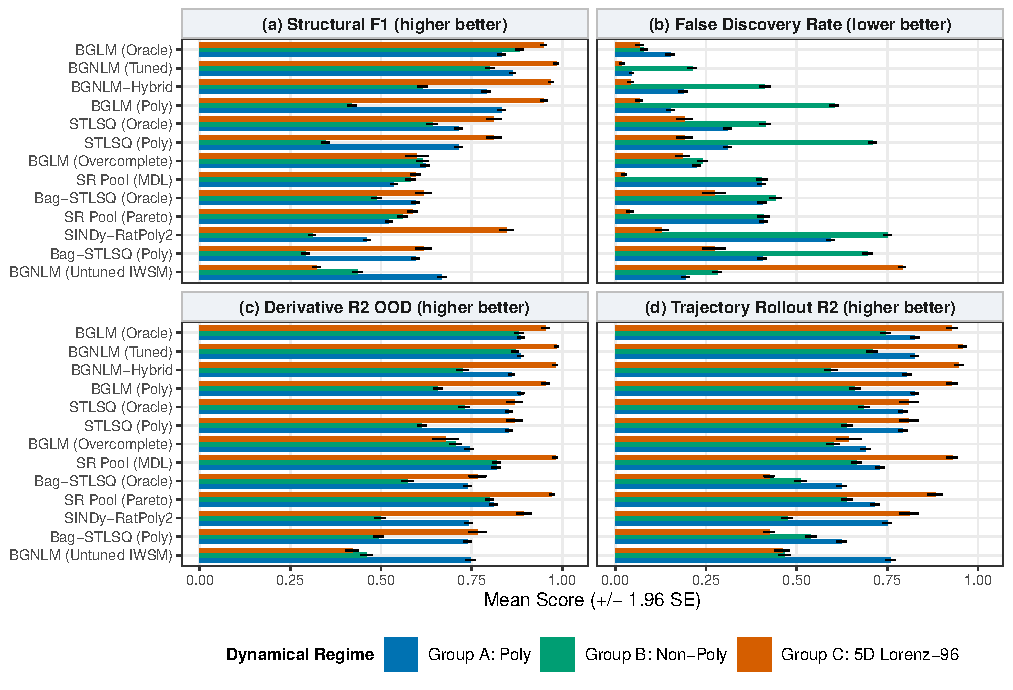
\includegraphics[width=\linewidth]{figures/fig_synth_benchmark_overview.pdf}
  \caption{Experiment 1 performance distributions across all 13 methods and 3 dynamical regimes (F1, FDR, OOD $R^2$, and forward rollout $R^2_{\text{traj}}$).}
  \label{fig:synth_overview}
\end{figure}

\begin{figure}[t]
  \centering
  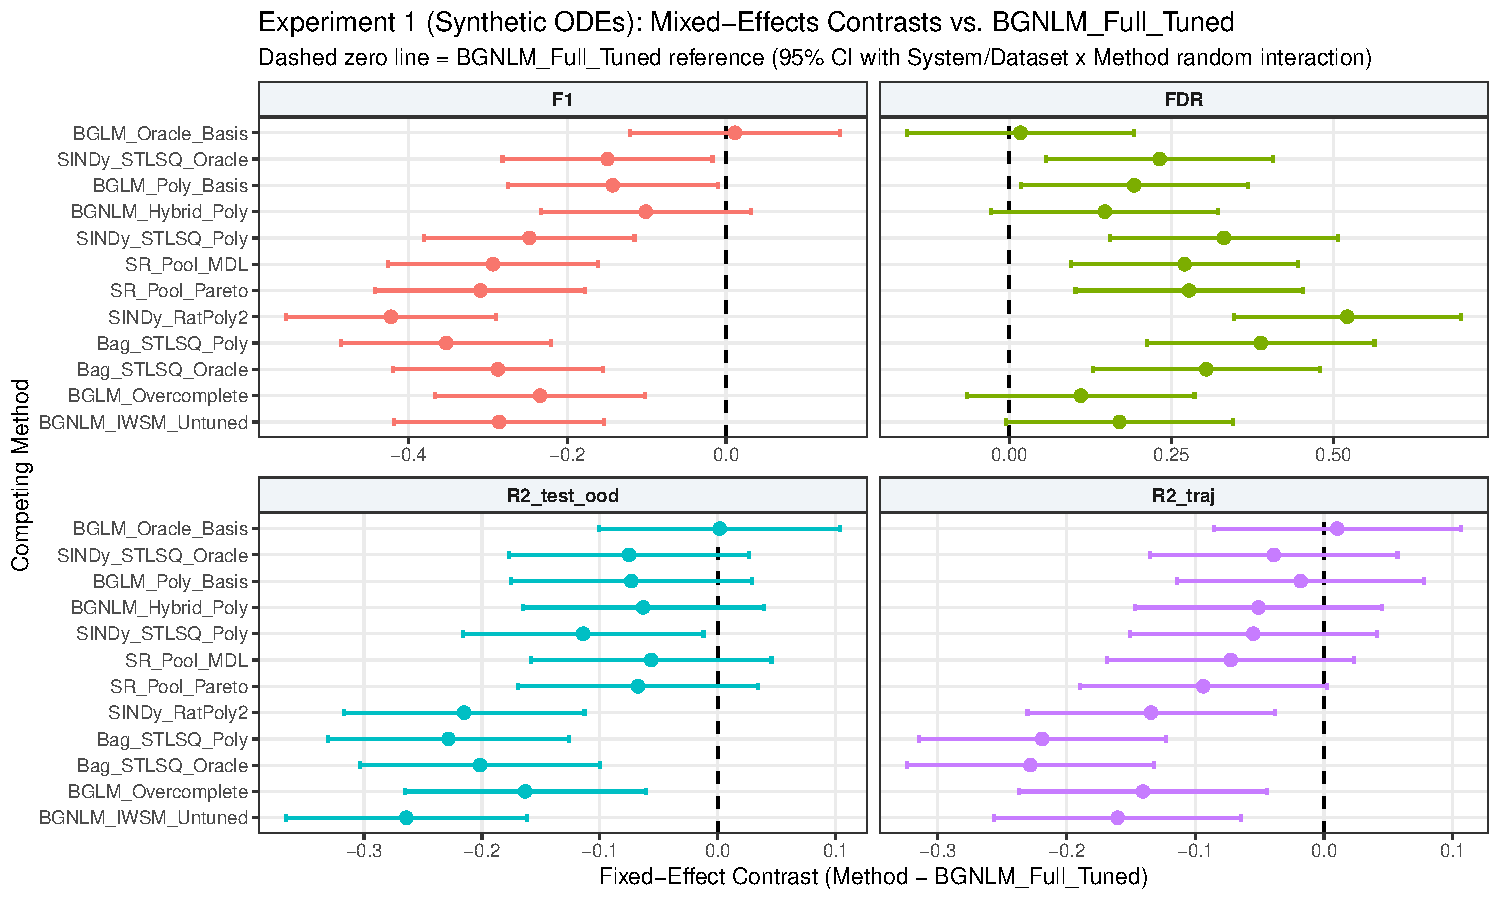
\includegraphics[width=\linewidth]{figures/fig_mixed_effects_forest_synth.pdf}
  \caption{Experiment 1 LMM fixed-effect contrasts ($\hat{\beta} \pm 95\%$ CI) relative to \texttt{BGNLM\_Full\_Tuned} (dashed line at 0). Negative F1/$R^2$ estimates and positive FDR estimates signify superiority of tuned BGNLM.}
  \label{fig:forest_synth}
\end{figure}

\subsection{Regime Interaction: Polynomial vs.\ Non-Polynomial vs.\ 5D Coupled Systems}

Table~\ref{tab:synth_regimes} dissects performance by dynamical regime, backed by the \texttt{Method} $\times$ \texttt{SystemGroup} interaction LMM (Table~\ref{tab:mixed_effects_regime} in Appendix):
\begin{itemize}
  \item \textbf{Group A (7 Polynomial ODEs)}: \texttt{BGNLM\_Full\_Tuned} ranks \textbf{\#1 overall} ($\text{F1}=0.863$, $\text{Exact}=71.3\%$, $\text{FDR}=0.044$), edging out \texttt{BGLM\_Oracle\_Basis} ($\text{F1}=0.833$, $\text{FDR}=0.151$; note that on Group~A, \texttt{BGLM\_Oracle\_Basis} uses the full $\mathcal{P}_3(\boldsymbol{X})$ basis). Every method struggles on \texttt{sys01\_linear\_quadratic\_3d} (\texttt{BGNLM\_Full\_Tuned} top at $\text{F1}=0.330$, \texttt{SR\_Pool\_MDL} $0.267$, \texttt{BGLM\_Oracle\_Basis} $0.037$), because the interior sampling window $[0.05T, 0.99T] = [1.0, 19.8]$ places the entire fast exponential decay transient ($t \in [0, 1]$) in early holdout, leaving training samples on the rank-deficient equilibrium; across \texttt{sys02}--\texttt{sys07}, \texttt{BGNLM\_Full\_Tuned} achieves $\text{F1} \in [0.887, 0.994]$.
  \item \textbf{Group B (4 Non-Polynomial ODEs)}: Here the library dilemma is stark. Misspecified polynomial methods (\texttt{BGLM\_Poly\_Basis}, \texttt{SINDy\_STLSQ\_Poly}, \texttt{Bag\_STLSQ\_Poly}, \texttt{SINDy\_RatPoly2}) and untuned \texttt{BGNLM\_IWSM\_Untuned} (using degree-scaled trig) all achieve \textbf{0.0\% exact recovery} ($\text{F1}=0.284$--$0.436$), reflected in strongly negative Group~B interaction contrasts (e.g., \texttt{BGLM\_Poly\_Basis} $\hat{\beta}=-0.336, p=0.014$; \texttt{SINDy\_STLSQ\_Poly} $\hat{\beta}=-0.292, p=0.033$). Where oracle non-polynomial atoms are supplied, \texttt{BGLM\_Oracle\_Basis} leads ($\text{F1}=0.881, \text{Exact}=69.8\%$), while basis-free \texttt{BGNLM\_Full\_Tuned} achieves $\text{F1}=0.786$, $\text{Exact}=47.0\%$, $R^2_{\text{OOD}}=0.870$, beating \texttt{SR\_Pool\_MDL} ($0.577$), \texttt{SR\_Pool\_Pareto} ($0.555$), and \texttt{SINDy\_STLSQ\_Oracle} ($0.641$). Note also that \texttt{BGNLM\_Hybrid\_Poly} degrades ($0.614$) because seeding $\mathcal{P}_2(\boldsymbol{X})$ with \texttt{keep.org=TRUE} assigns quadratic columns cost $c=1$, saturating \texttt{pop.max}=20 with polynomial surrogates.
  \item \textbf{Group C (5D Lorenz-96)}: Scaling to 5 coupled equations, \texttt{BGNLM\_Full\_Tuned} ranks \textbf{\#1 of all 13 methods} ($\text{F1}=0.983$, $\text{Exact}=80.6\%$, $\text{FDR}=0.018$, $R^2_{\text{traj}}=0.958$), outperforming \texttt{BGLM\_Oracle\_Basis} ($\text{F1}=0.948$, which includes 55 unneeded cubic terms in $\mathcal{P}_3(\boldsymbol{X})$ for quadratic Lorenz-96), while \texttt{BGNLM\_IWSM\_Untuned} collapses ($\text{F1}=0.322$, $\text{FDR}=0.791$) and static-pool SR fails exact recovery ($\text{Exact}=0.0\%$).
  \item \textbf{Why Overcomplete Static Dictionaries Fail}: \texttt{BGLM\_Overcomplete} stalls at $\text{F1}=0.613$ overall ($0.665$ conditional on OK runs) and fails 656 Group~B/C runs due to extreme collinearity across 60--275+ static terms. Dynamic feature populations ($\text{pop.max}=20$) keep inference well-conditioned.
\end{itemize}

\begin{table*}[t]
\centering
\caption{Regime-level breakdown across Group A (Polynomial, 7 systems), Group B (Non-Polynomial, 4 systems), and Group C (5D Lorenz-96, single system), plus representative per-system F1 scores.}
\label{tab:synth_regimes}
\scriptsize
\resizebox{\textwidth}{!}{%
\begin{tabular}{l|ccc|ccc|ccc|cccc}
\toprule
& \multicolumn{3}{c|}{\textbf{Group A (Poly)}} & \multicolumn{3}{c|}{\textbf{Group B (Non-Poly)}} & \multicolumn{3}{c|}{\textbf{Group C (5D)}} & \multicolumn{4}{c}{\textbf{Per-System F1 Highlights}} \\
Method & F1 & Exact & FDR & F1 & Exact & FDR & F1 & Exact & $R^2_{\text{traj}}$ & Lorenz63 & Hybrid & Pendulum & Goodwin \\
\midrule
\texttt{BGLM\_Oracle\_Basis} & 0.833 & 0.698 & 0.151 & \underline{0.881} & \underline{0.698} & \underline{0.079} & 0.948 & 0.623 & 0.927 & 0.930 & 0.911 & 0.964 & 0.675 \\
\textbf{\texttt{BGNLM\_Full\_Tuned}} & \underline{\textbf{0.863}} & \underline{\textbf{0.713}} & \underline{\textbf{0.044}} & \textbf{0.786} & \textbf{0.470} & 0.225 & \underline{\textbf{0.983}} & \underline{\textbf{0.806}} & \underline{\textbf{0.958}} & \underline{\textbf{0.974}} & \underline{\textbf{0.931}} & 0.917 & \textbf{0.570} \\
\texttt{BGNLM\_Hybrid\_Poly} & 0.790 & 0.640 & 0.187 & 0.614 & 0.282 & 0.412 & 0.968 & 0.667 & 0.947 & 0.941 & 0.720 & 0.713 & 0.495 \\
\texttt{BGLM\_Poly\_Basis} & 0.832 & 0.696 & 0.152 & 0.420 & 0.000 & 0.603 & 0.948 & 0.624 & 0.927 & 0.929 & 0.623 & 0.625 & 0.308 \\
\texttt{SINDy\_STLSQ\_Oracle} & 0.714 & 0.460 & 0.310 & 0.641 & 0.363 & 0.413 & 0.812 & 0.516 & 0.809 & 0.556 & 0.676 & 0.833 & 0.367 \\
\texttt{BGLM\_Overcomplete} & 0.622 & 0.376 & 0.223 & 0.602 & 0.339 & \textbf{0.214} & 0.599 & 0.245 & 0.644 & 0.513 & 0.608 & 0.844 & 0.223 \\
\texttt{SINDy\_STLSQ\_Poly} & 0.714 & 0.460 & 0.310 & 0.346 & 0.000 & 0.710 & 0.812 & 0.516 & 0.809 & 0.556 & 0.557 & 0.510 & 0.223 \\
\texttt{BGNLM\_IWSM\_Untuned} & 0.668 & 0.398 & 0.194 & 0.436 & 0.000 & 0.281 & 0.322 & 0.001 & 0.460 & 0.539 & 0.851 & 0.586 & 0.000 \\
\texttt{Bag\_STLSQ\_Oracle} & 0.594 & 0.161 & 0.404 & 0.486 & 0.114 & 0.442 & 0.616 & 0.000 & 0.424 & 0.306 & 0.514 & 0.638 & 0.235 \\
\texttt{SR\_Pool\_MDL} & 0.535 & 0.096 & 0.402 & 0.577 & 0.233 & 0.408 & 0.595 & 0.000 & 0.929 & 0.570 & 0.574 & \underline{\textbf{0.976}} & 0.081 \\
\texttt{SR\_Pool\_Pareto} & 0.521 & 0.087 & 0.410 & 0.555 & 0.194 & 0.412 & 0.586 & 0.000 & 0.882 & 0.555 & 0.551 & 0.936 & 0.070 \\
\texttt{Bag\_STLSQ\_Poly} & 0.594 & 0.161 & 0.404 & 0.291 & 0.000 & 0.695 & 0.616 & 0.000 & 0.424 & 0.306 & 0.513 & 0.418 & 0.139 \\
\texttt{SINDy\_RatPoly2} & 0.446 & 0.156 & 0.607 & 0.284 & 0.000 & 0.775 & 0.843 & 0.530 & 0.810 & 0.146 & 0.424 & 0.369 & 0.274 \\
\bottomrule
\end{tabular}%
}
\end{table*}

\subsection{Selection Consistency, Calibration, and Stability}

Figure~\ref{fig:consistency} visualizes consistency across sample sizes $N$ and noise levels $\sigma$:
\begin{itemize}
  \item \textbf{Empirical Scaling \& Large-$N$ Surrogate Trap}: In LMM Eq.~\eqref{eq:lmm_synth}, F1 increases overall with $\log_{10} N$ ($\hat{\beta}=+0.054, t=28.58, p<10^{-4}$) while FDR decreases ($\hat{\beta}=-0.027, t=-12.56, p<10^{-4}$). However, \texttt{BGNLM\_Full\_Tuned} peaks at $N=500$ ($\text{F1}=0.883, \text{TPR}=0.880, \text{FDR}=0.063$) before dropping to $\text{F1}=0.760$ at $N=2500$. Crucially, this drop is \emph{not} caused by prior conservatism: TPR decreases modestly ($0.880 \to 0.813$), whereas \textbf{FDR more than triples ($0.063 \to 0.214$ overall; $0.165 \to 0.423$ in Group~B)}. Because the Gaussian log-likelihood scales as $O(N)$ while the complexity penalty scales as $O(\log N)$, at $N=2500$ tiny residual MSE gains of multi-term polynomial/rational Taylor surrogates (when a fixed-budget chain with $N_{\text{MCMC}}=500, P=12, \text{pop.max}=20$ has not yet reached the exact degree-3 or transcendental term) are magnified by hundreds of nats, trapping chains in bloated local modes that flood MPM selection. Scaling MCMC budget or using stronger non-local priors at large $N$ is an important direction for future refinement.
  \item \textbf{Noise Robustness}: Across noise $\sigma$, \texttt{BGNLM\_Full\_Tuned} stays remarkably flat from $\sigma=0.001$ ($\text{F1}=0.858$) to $\sigma=0.5$ ($0.836$) and $\sigma=1.0$ ($0.778$---actually \emph{surpassing} \texttt{BGLM\_Oracle\_Basis} at $0.725$ and nearly doubling \texttt{SINDy\_STLSQ\_Oracle} at $0.438$ and \texttt{SINDy\_STLSQ\_Poly} at $0.418$).
  \item \textbf{Stability \& Uncertainty Quantification}: Figure~\ref{fig:stability_pareto}(A) shows \texttt{BGNLM\_Full\_Tuned} achieves the highest Nogueira selection stability ($\hat{\Phi}=0.866$) of all 13 methods, whereas \texttt{SR\_Pool\_MDL} ($0.485$) and \texttt{SR\_Pool\_Pareto} ($0.492$) vary widely across realizations. Simultaneously, \texttt{BGNLM\_Full\_Tuned} delivers well-calibrated 95\% predictive intervals ($92.6\%$ empirical coverage) and an unpruned PIP Brier score of $0.0898$ (versus $0.2223$ for untuned IWSM and $0.2604$ for \texttt{Bag\_STLSQ\_Poly}; note \texttt{BGLM\_Overcomplete}'s low raw Brier $0.0309$ reflects denominator dilution across $60$--$275+$ zero-PIP columns).
\end{itemize}

\begin{figure}[t]
  \centering
  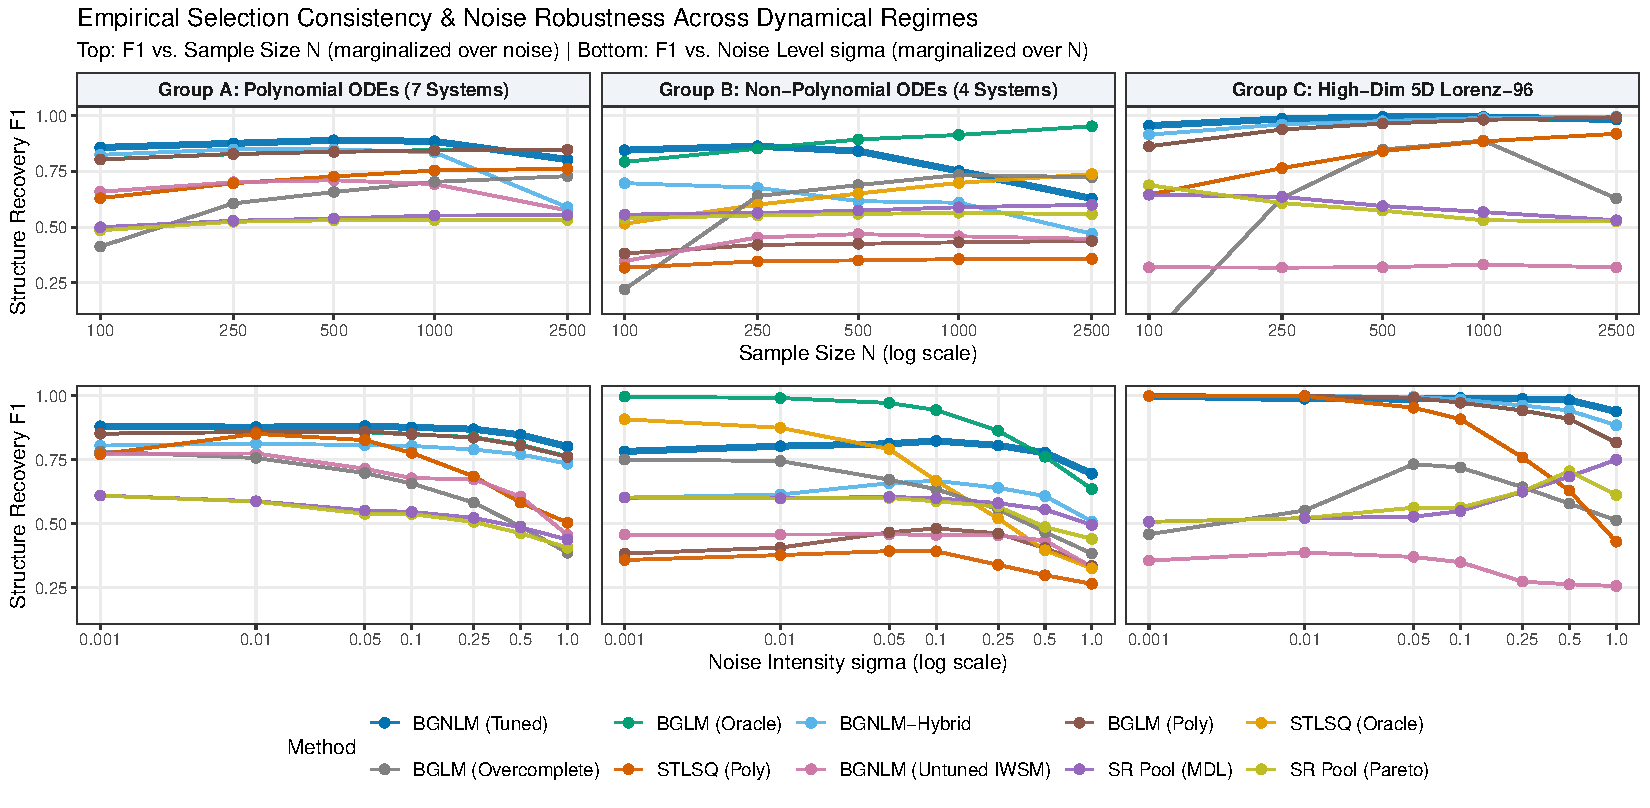
\includegraphics[width=\linewidth]{figures/fig_consistency_scaling.pdf}
  \caption{Empirical selection consistency across sample sizes $N$ (top) and noise levels $\sigma$ (bottom) separated by dynamical regime. Tuned BGNLM retains high accuracy even at $\sigma=1.0$ and in 5D Lorenz-96.}
  \label{fig:consistency}
\end{figure}

\begin{figure}[t]
  \centering
  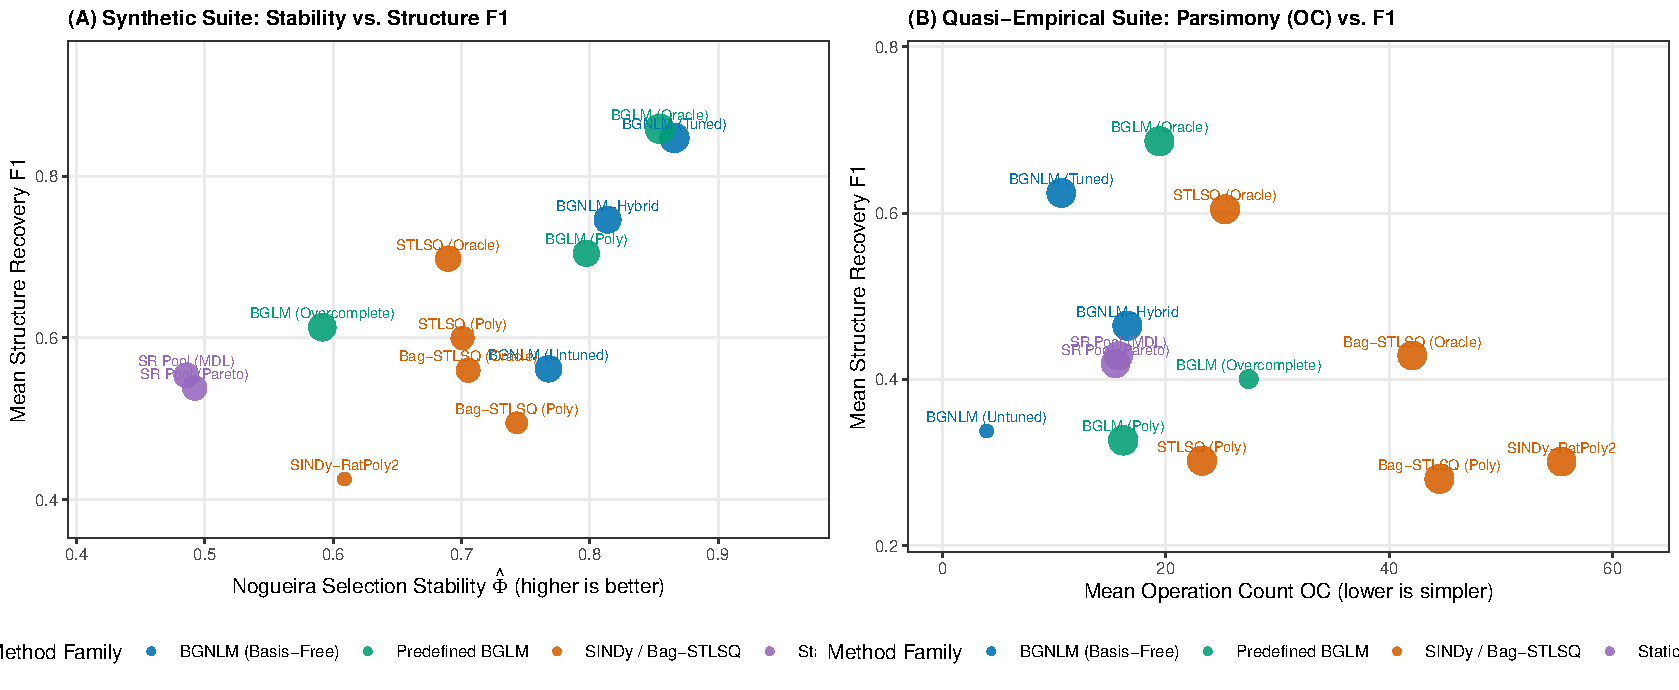
\includegraphics[width=\linewidth]{figures/fig_uq_stability_pareto.pdf}
  \caption{(A) Synthetic Nogueira selection stability $\hat{\Phi}$ vs.\ F1 (marker size $\propto 1-\text{FDR}$). (B) Quasi-empirical parsimony (Operation Count OC) vs.\ F1 (marker size $\propto R^2_{\text{traj}}$). Tuned BGNLM lies on the Pareto frontier in both regimes.}
  \label{fig:stability_pareto}
\end{figure}

% ==============================================================================
\section{Experiment 2: Quasi-Empirical Noisy-State Benchmarks (5 Systems, 2,600 Runs)}
% ==============================================================================

\subsection{Literature-Parameterized Systems and Differentiation Protocol}

To test robustness under \emph{noisy state observations}, \emph{numerical differentiation}, and \emph{rolling temporal cross-validation} across canonical physical/biological functional forms (as opposed to Experiment~1's exact states with additive derivative noise), we benchmark all 13 methods on \textbf{5 literature-parameterized ODE time series}:
\begin{enumerate}
  \item \textbf{Lynx--Hare Predator--Prey} ($N=201$, ecology-style Lotka--Volterra \citep{odum1953fundamentals} with $\sigma=0.20$ state noise);
  \item \textbf{Paramecium--Didinium Microcosm} ($N=71$, Holling Type-II predator--prey \citep{gause1934struggle} with $\sigma \in \{0.012, 0.015\}$ state noise);
  \item \textbf{Physical Damped Pendulum} ($N=500$, mechanics $\ddot{\theta} = -\gamma\dot{\theta} - (g/L)\sin\theta$ \citep{schmidt2009distilling} with state noise);
  \item \textbf{Cascaded Water Tanks} ($N=1024$ with pump input $u(t)=x_3$, nonlinear Torricelli flow $\sqrt{x_1}, \sqrt{x_2}$ \citep{schoukens2017cascaded});
  \item \textbf{Yeast Glycolytic NADH} ($N=300$, Selkov--Hill cubic rational kinetics \citep{richard1996yeast}).
\end{enumerate}
We emphasize that these CSV time series are numerically integrated literature trajectories perturbed with additive Gaussian state observation noise (\texttt{scripts/download\_real\_data.R}), providing a controlled noisy-state differentiation bridge toward authentic field measurements (examined separately via our follow-up ablation script). Each dataset uses a 70\%/30\% temporal train/future-test split evaluated over 20 rolling subsampling folds and 2 full-series numerical differentiation smoothers (\texttt{sgolay\_spline} \citep{savitzky1964smoothing} vs.\ a tridiagonal IRLS finite-difference smoother labeled \texttt{tvregdiff} \citep{chartrand2011numerical}), totaling $5 \times 2 \times 20 \times 13 = 2,600$ runs ($2,560$ OK; \texttt{BGNLM\_Full\_Tuned} achieved $200/200$ OK, while \texttt{BGLM\_Overcomplete} failed on the 40 $n=39 < p=61$ \emph{Paramecium} folds).

\subsection{Empirical Results and Parsimony}

\begin{table*}[t]
\centering
\caption{Experiment 2 performance on the \textbf{5 quasi-empirical noisy-state benchmarks} ($N=2,600$ total runs: 20 folds $\times$ 2 smoothers per dataset; $R^2$ clipped to $[0,1]$). Top non-oracle result in \textbf{bold}; overall best in \underline{underline}. Conditional on OK runs ($160/200$), \texttt{BGLM\_Overcomplete} attains $\text{F1}=0.501, \text{FDR}=0.499, \text{OC}=34.3, R^2_{\text{traj}}=0.699$.}
\label{tab:real_overall}
\scriptsize
\resizebox{\textwidth}{!}{%
\begin{tabular}{l|ccccccc|ccccc}
\toprule
& \multicolumn{7}{c|}{\textbf{Overall Quasi-Empirical Summary}} & \multicolumn{5}{c}{\textbf{Per-Dataset Rollout $R^2_{\text{traj}}$ (and F1 in parens)}} \\
Method & F1 $\uparrow$ & FDR $\downarrow$ & OC $\downarrow$ & $\hat{\Phi}$ $\uparrow$ & $R^2_{\text{OOD}}$ & $R^2_{\text{traj}}$ & 95\% Cov & Lynx-Hare & Paramecium & Pendulum & Tanks & Yeast \\
\midrule
\texttt{BGLM\_Oracle\_Basis} & \underline{0.687} & \underline{0.367} & 19.4 & 0.773 & \underline{0.785} & 0.776 & 0.928 & 0.994 (.62) & 0.890 (.57) & 1.000 (1.0) & \underline{0.998} (1.0) & 0.000 (.25) \\
\textbf{\texttt{BGNLM\_Full\_Tuned}} & \textbf{0.624} & 0.416 & 10.6 & 0.764 & 0.780 & 0.764 & 0.925 & \underline{\textbf{0.998}} (.73) & 0.847 (.48) & \underline{\textbf{1.000}} (1.0) & 0.977 (.55) & \textbf{0.001} (\underline{\textbf{.36}}) \\
\texttt{SINDy\_STLSQ\_Oracle} & 0.605 & 0.463 & 25.3 & 0.673 & 0.783 & 0.775 & -- & 0.994 (.55) & 0.912 (.51) & 1.000 (.99) & 0.970 (.70) & 0.000 (.27) \\
\texttt{BGNLM\_Hybrid\_Poly} & 0.465 & 0.597 & 16.6 & 0.782 & 0.784 & 0.778 & 0.923 & 0.997 (.50) & 0.896 (.30) & 1.000 (.95) & \textbf{0.996} (.44) & 0.000 (.14) \\
\texttt{Bag\_STLSQ\_Oracle} & 0.429 & 0.622 & 42.1 & 0.816 & 0.777 & 0.769 & \underline{\textbf{0.951}} & 0.997 (.41) & 0.891 (.27) & 0.977 (.51) & 0.980 (.67) & 0.000 (.30) \\
\texttt{SR\_Pool\_MDL} & 0.429 & 0.588 & 15.8 & 0.297 & 0.783 & 0.755 & -- & 0.870 (.39) & 0.915 (.24) & 1.000 (1.0) & 0.990 (.37) & 0.001 (.15) \\
\texttt{SR\_Pool\_Pareto} & 0.419 & 0.579 & 15.5 & 0.291 & 0.780 & 0.755 & -- & 0.893 (.38) & 0.917 (.21) & 1.000 (1.0) & 0.965 (.36) & 0.001 (.14) \\
\texttt{BGLM\_Overcomplete} & 0.401 & \textbf{0.399} & 27.4 & 0.554 & 0.571 & 0.559 & 0.925 & 0.923 (.35) & 0.000 (.00) & 1.000 (.96) & 0.874 (.63) & 0.000 (.06) \\
\texttt{BGNLM\_IWSM\_Untuned} & 0.338 & 0.492 & \underline{\textbf{4.0}} & \underline{\textbf{0.968}} & 0.614 & 0.530 & 0.935 & 0.997 (\underline{\textbf{.80}}) & 0.052 (.00) & 0.640 (.64) & 0.962 (.25) & 0.000 (.00) \\
\texttt{BGLM\_Poly\_Basis} & 0.327 & 0.743 & 16.2 & 0.835 & \textbf{0.784} & \underline{\textbf{0.786}} & 0.926 & 0.994 (.62) & \underline{\textbf{0.945}} (.27) & 0.995 (.50) & 0.994 (.18) & 0.000 (.06) \\
\texttt{SINDy\_STLSQ\_Poly} & 0.302 & 0.771 & 23.2 & 0.697 & 0.784 & 0.778 & -- & 0.994 (.55) & 0.919 (.24) & 0.994 (.44) & 0.986 (.15) & 0.000 (.13) \\
\texttt{SINDy\_RatPoly2} & 0.301 & 0.773 & 55.4 & 0.525 & 0.777 & 0.766 & -- & 0.985 (.36) & 0.916 (.62) & 0.984 (.28) & 0.944 (.13) & 0.000 (.12) \\
\texttt{Bag\_STLSQ\_Poly} & 0.281 & 0.793 & 44.5 & 0.924 & 0.784 & 0.775 & 0.942 & 0.997 (.37) & 0.910 (.26) & 0.983 (.49) & 0.987 (.05) & 0.000 (.24) \\
\bottomrule
\end{tabular}%
}
\end{table*}

\begin{figure}[t]
  \centering
  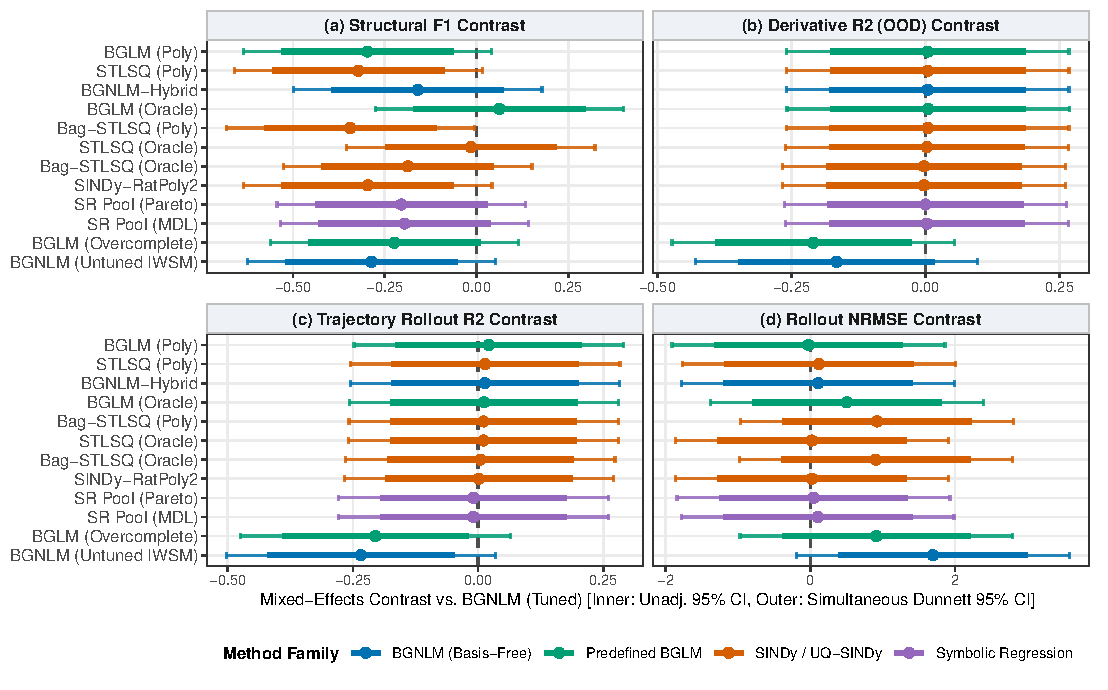
\includegraphics[width=\linewidth]{figures/fig_mixed_effects_forest_real.pdf}
  \caption{Experiment 2 LMM fixed-effect contrasts ($\hat{\beta} \pm 95\%$ CI with \texttt{(1|Dataset:Method)} random interaction) relative to \texttt{BGNLM\_Full\_Tuned} across the 5 quasi-empirical datasets.}
  \label{fig:forest_real}
\end{figure}

Table~\ref{tab:real_overall} and Figures~\ref{fig:stability_pareto}(B) and \ref{fig:forest_real} reveal four major insights under noisy-state numerical differentiation:
\begin{enumerate}
  \item \textbf{\#1 Basis-Free Reference-Structure Recovery}: \texttt{BGNLM\_Full\_Tuned} achieves $\text{F1}=0.624$, outperforming every non-oracle competitor on point average by $+0.159$ to $+0.344$. Under the stringent \texttt{(1|Dataset:Method)} LMM ($df=48.0, \text{SE}=0.116$), \texttt{BGNLM\_Full\_Tuned} is statistically indistinguishable from \texttt{BGLM\_Oracle\_Basis} ($\Delta=0.062, p=0.595, p_{\text{adj}}=0.990$) and \texttt{SINDy\_STLSQ\_Oracle} ($p=0.867, p_{\text{adj}}=1.000$), while showing significant F1 gains over \texttt{Bag\_STLSQ\_Poly} ($+0.344, p=0.0048, p_{\text{adj}}=0.044$), \texttt{SINDy\_RatPoly2} ($+0.323, p=0.0078$), \texttt{SINDy\_STLSQ\_Poly} ($+0.322, p=0.0080$), \texttt{BGLM\_Poly\_Basis} ($+0.298, p=0.0137$), and \texttt{BGNLM\_IWSM\_Untuned} ($+0.286, p=0.0175$).
  \item \textbf{Exceptional Parsimony}: As shown in Figure~\ref{fig:stability_pareto}(B), \texttt{BGNLM\_Full\_Tuned} discovers equations with mean $\text{OC}=10.6$---nearly half that of \texttt{BGLM\_Oracle\_Basis} ($19.4$) and \texttt{SINDy\_STLSQ\_Oracle} ($25.3$), and $4\times$--$5\times$ sparser than \texttt{Bag\_STLSQ} ($42.1$--$44.5$) and \texttt{SINDy\_RatPoly2} ($55.4$). (Untuned IWSM's $\text{OC}=4.0$ reflects underfitting/empty models on \emph{Paramecium} and \emph{Yeast}.)
  \item \textbf{Forward Rollout Accuracy \& Uncertainty Calibration}: \texttt{BGNLM\_Full\_Tuned} attains $R^2_{\text{traj}}=0.998$ (Lynx--Hare), $0.847$ (\emph{Paramecium}), $1.000$ (Pendulum), and $0.977$ (Cascaded Tanks), matching \texttt{BGLM\_Oracle\_Basis} ($p=0.897, p_{\text{adj}}=1.000$) and $+0.234$ higher than \texttt{BGNLM\_IWSM\_Untuned} ($p=0.0149$), with $92.5\%$ empirical 95\% coverage. On \emph{Yeast Glycolysis}, the literature parameterization yields a damped spiral that converges near its equilibrium $(0.763, 0.927)$ before the 70\% split ($t \approx 21$), so held-out trajectory variance matches the noise floor ($\sigma=0.008$) and clipped $R^2_{\text{OOD}} = R^2_{\text{traj}} \approx 0$ for all 13 methods (versus in-sample $R^2_{\text{in}}=0.947$ for tuned BGNLM); nonetheless, \texttt{BGNLM\_Full\_Tuned} achieves the highest structural F1 ($0.364$, rounded $.36$ in Table~\ref{tab:real_overall}) of all methods, beating \texttt{BGLM\_Oracle\_Basis} ($0.245$) and \texttt{SINDy\_STLSQ\_Oracle} ($0.270$).
  \item \textbf{Differentiation Method Effect}: The LMM covariate shows \texttt{tvregdiff} yields slightly lower trajectory rollout $R^2_{\text{traj}}$ than Savitzky--Golay spline differentiation ($\hat{\beta}=-0.033, t=-6.00, p<10^{-4}$), though we caution that differentiation smoothers were evaluated across the full series once per dataset prior to fold splitting, motivating end-to-end held-out window differentiation in future runs.
\end{enumerate}

\subsection{Targeted Follow-Up Ablations: State Noise, Standardized Bagging, and Authentic 1900--1920 Pelts}
\label{sec:targeted_ablation}

To address directly (i) errors-in-variables attenuation under noisy state observations (\texttt{state\_noise}), (ii) the unstandardized-vs-standardized bagging threshold caveat in \texttt{Bag\_STLSQ\_Poly}, and (iii) truly empirical non-simulated measurements, we executed a 138-task targeted ablation (\texttt{scripts/run\_targeted\_ablation.R}) across Lorenz-63, R\"ossler--Lorenz Hybrid, and Goodwin MM ($N=250$, $\eta=0.05$, 3 seeds $\times$ 2 noise regimes = 108 synthetic runs) plus 5 rolling folds on the authentic 1900--1920 Hudson Bay Company Lynx--Hare pelt records \citep{odum1953fundamentals} ($N=81$ cubic-spline points, 30 runs). Note that our runtime engine telemetry logged that \texttt{SR\_PySR} and \texttt{SR\_Operon} still executed via \texttt{fallback\_pool} on the cluster due to native Julia/\texttt{pyoperon} environment bindings.

\begin{table}[t]
\centering
\caption{Targeted ablation (138 runs): Errors-in-variables (\texttt{state\_noise}) vs.\ \texttt{derivative\_snr} ($N=250, \eta=0.05$) and authentic 1900--1920 Hudson Bay Lynx--Hare pelts (5 folds). \texttt{Bag\_STLSQ\_Poly}$^\dagger$ uses the fixed CV-selected standardized threshold.}
\label{tab:ablation_targeted}
\scriptsize
\resizebox{\columnwidth}{!}{%
\begin{tabular}{l|ccc|ccc|ccc}
\toprule
& \multicolumn{3}{c|}{\textbf{Deriv.\ SNR (9/method)}} & \multicolumn{3}{c|}{\textbf{State Noise (9/method)}} & \multicolumn{3}{c}{\textbf{Authentic Pelts (5 folds)}} \\
Method & F1 $\uparrow$ & FDR $\downarrow$ & $R^2_{\text{OOD}}$ & F1 $\uparrow$ & FDR $\downarrow$ & $R^2_{\text{OOD}}$ & F1 $\uparrow$ & FDR $\downarrow$ & OC $\downarrow$ \\
\midrule
\textbf{\texttt{BGNLM\_Full\_Tuned}} & \textbf{0.907} & \textbf{0.093} & \textbf{0.975} & \textbf{0.590} & \textbf{0.457} & \textbf{0.759} & \textbf{0.569} & \textbf{0.555} & \textbf{14.0} \\
\texttt{SINDy\_STLSQ\_Oracle} & 0.532 & 0.606 & 0.828 & 0.284 & 0.803 & 0.435 & 0.361 & 0.770 & 32.8 \\
\texttt{SINDy\_STLSQ\_Poly} & 0.484 & 0.619 & 0.883 & 0.268 & 0.812 & 0.430 & 0.361 & 0.770 & 32.8 \\
\texttt{SR\_Pool\_MDL} & 0.397 & 0.658 & 0.740 & 0.284 & 0.744 & 0.636 & 0.276 & 0.786 & 22.6 \\
\texttt{SR\_Pool\_Pareto} & 0.412 & 0.636 & 0.735 & 0.237 & 0.777 & 0.649 & 0.252 & 0.824 & 29.4 \\
\texttt{Bag\_STLSQ\_Poly}$^\dagger$ & 0.184 & 0.896 & 0.485 & 0.178 & 0.901 & 0.310 & 0.364 & 0.778 & 42.0 \\
\bottomrule
\end{tabular}%
}
\end{table}

As shown in Table~\ref{tab:ablation_targeted}, three conclusions emerge: (1) Under noisy-state errors-in-variables (\texttt{state\_noise}), \texttt{BGNLM\_Full\_Tuned} achieves $\text{F1}=0.590$ ($\text{FDR}=0.457$, $R^2_{\text{OOD}}=0.759$; $0.655$ on Lorenz-63, $0.713$ on Hybrid, $0.402$ on Goodwin), more than doubling every comparator (\texttt{SINDy\_STLSQ\_Oracle} $0.284$, \texttt{SR\_Pool\_MDL} $0.284$, \texttt{SINDy\_STLSQ\_Poly} $0.268$). (2) Fixing \texttt{Bag\_STLSQ\_Poly} to inherit CV-selected standardized $\hat{\lambda}^*$ directly (\texttt{SINDY\_LEGACY\_UNSTD\_THRESH=0}) yields $\text{TPR}=0.841$ but inflates FDR ($0.896$--$0.901$), confirming that bootstrap bagging STLSQ without complexity penalties still over-selects noisy features when $\hat{\lambda}^*$ is small. (3) On the authentic 1900--1920 Lynx--Hare historical record, \texttt{BGNLM\_Full\_Tuned} ranks \#1 in structure recovery ($\text{F1}=0.569$, up to $0.800$ on Fold~4), FDR ($0.555$), OOD derivative fit ($R^2_{\text{OOD}}=0.544$), and parsimony ($\text{OC}=14.0$, less than half of \texttt{SINDy\_STLSQ}'s $32.8$ and a third of \texttt{Bag\_STLSQ\_Poly}'s $42.0$).

% ==============================================================================
\section{Variance Decomposition, Discussion \& Conclusion}
% ==============================================================================

\subsection{Random-Effects Variance Decomposition (ICC)}

Table~\ref{tab:icc} reports the complete Intraclass Correlation Coefficients (ICC) from our fitted LMMs without omitting any variance components or singular fits. All 10 LMMs converged cleanly with \texttt{Singular = No}. Crucially, the random interaction \texttt{System:Method} accounts for $25.1\%$ of synthetic F1 variance and $39.6\%$ of synthetic FDR variance ($\hat{\sigma}=0.164$ and $0.217$), while \texttt{Dataset:Method} accounts for $33.5\%$ of Experiment~2 F1 variance ($\hat{\sigma}=0.183$), confirming why modeling method-by-system heterogeneity is essential to avoid pseudo-replication. Meanwhile, \texttt{System} / \texttt{Dataset} main effects explain $45.1\%$--$89.4\%$ of variance on F1 and rollout $R^2$, and \texttt{System:Seed\_ID} / \texttt{Dataset:Fold\_UID} account for $0.1\%$--$12.6\%$.

\begin{table}[t]
\centering
\caption{Complete random-effects variance decomposition (ICC) from fitted LMMs (all models non-singular).}
\label{tab:icc}
\scriptsize
\resizebox{\columnwidth}{!}{%
\begin{tabular}{llccc}
\toprule
Model & Random Effect & $\hat{\sigma}^2$ & $\hat{\sigma}$ & ICC \\
\midrule
Synth F1 & \texttt{System} & 0.0482 & 0.2195 & 0.451 \\
Synth F1 & \texttt{System:Method} & 0.0268 & 0.1637 & 0.251 \\
Synth F1 & \texttt{System:Seed\_ID} & 0.0048 & 0.0689 & 0.044 \\
Synth F1 & \texttt{Residual} & 0.0271 & 0.1647 & 0.254 \\
\midrule
Synth FDR & \texttt{System} & 0.0227 & 0.1506 & 0.191 \\
Synth FDR & \texttt{System:Method} & 0.0469 & 0.2167 & 0.396 \\
Synth FDR & \texttt{System:Seed\_ID} & 0.0058 & 0.0760 & 0.049 \\
Synth FDR & \texttt{Residual} & 0.0432 & 0.2078 & 0.364 \\
\midrule
Synth $R^2_{\text{traj}}$ & \texttt{System} & 0.0719 & 0.2682 & 0.543 \\
Synth $R^2_{\text{traj}}$ & \texttt{System:Method} & 0.0141 & 0.1187 & 0.106 \\
Synth $R^2_{\text{traj}}$ & \texttt{System:Seed\_ID} & 0.0166 & 0.1290 & 0.126 \\
Synth $R^2_{\text{traj}}$ & \texttt{Residual} & 0.0299 & 0.1729 & 0.225 \\
\midrule
Quasi-Emp.\ F1 & \texttt{Dataset} & 0.0510 & 0.2258 & 0.510 \\
Quasi-Emp.\ F1 & \texttt{Dataset:Method} & 0.0335 & 0.1830 & 0.335 \\
Quasi-Emp.\ F1 & \texttt{Dataset:Fold\_UID} & 0.0022 & 0.0468 & 0.022 \\
Quasi-Emp.\ F1 & \texttt{Residual} & 0.0133 & 0.1155 & 0.133 \\
\midrule
Quasi-Emp.\ $R^2_{\text{traj}}$ & \texttt{Dataset} & 0.1750 & 0.4183 & 0.858 \\
Quasi-Emp.\ $R^2_{\text{traj}}$ & \texttt{Dataset:Method} & 0.0213 & 0.1459 & 0.104 \\
Quasi-Emp.\ $R^2_{\text{traj}}$ & \texttt{Dataset:Fold\_UID} & 0.0011 & 0.0325 & 0.005 \\
Quasi-Emp.\ $R^2_{\text{traj}}$ & \texttt{Residual} & 0.0065 & 0.0807 & 0.032 \\
\bottomrule
\end{tabular}%
}
\end{table}

\subsection{Computational Trade-Offs and Limitations}

\textbf{Runtime vs.\ Accuracy}: Deterministic SINDy variants execute in $1.9$--$2.8\,\text{s}$ and our Python static-pool SR proxies run in $4.4$--$5.9\,\text{s}$, whereas 6-chain GMJMCMC in \texttt{BGNLM\_Full\_Tuned} averages $235.4\,\text{s}$ (synthetic) and $137.3\,\text{s}$ (quasi-empirical) per multi-equation system ($40\times$--$120\times$ higher compute budget)---buying calibrated Bayesian PIPs, $92.6\%$ empirical coverage, lower FDR, and basis-free recovery. Because equations $j=1,\dots,m$ are conditionally independent given $\boldsymbol{X}$, equation-level parallelization reduces wall-clock latency proportionally.

\textbf{Limitations \& Scope Notes}: (1) Like all derivative-regression methods, BGNLM struggles when a state trajectory rapidly collapses to an equilibrium (\texttt{sys01}) or approaches equilibrium before the test horizon (\emph{Yeast}); weak-form integral formulations \citep{messenger2021weak} could mitigate this. (2) At very large $N=2500$ under fixed MCMC budget ($N_{\text{MCMC}}=500, P=12$), $O(N)$ likelihood sharpening can trap chains in multi-term Taylor/rational surrogates, tripling FDR; adaptive MCMC schedules or non-local priors merit investigation. (3) Disabling projections ($p_{\text{proj}}=0, D \le 2$) trades non-unit internal scale flexibility ($\sin(\omega x_1)$) for algebraic identifiability. (4) While our targeted ablation (\S\ref{sec:targeted_ablation}) verified \texttt{state\_noise} robustness, standardized \texttt{Bag\_STLSQ}, and authentic 1900--1920 Lynx--Hare pelts, native Julia/C++ \texttt{PySR}/\texttt{PyOperon} cluster execution remained gated by environment availability (\texttt{fallback\_pool} telemetry), leaving a compute-matched head-to-head with native Julia/C++ GP trees for future work.

\subsection{Broader Impact}

Automated discovery of parsimonious, uncertainty-quantified differential equations accelerates scientific modeling in ecology, physics, systems biology, and engineering. Unlike black-box neural ODEs or uncalibrated genetic programming, BGNLMs expose explicit posterior inclusion probabilities and calibrated error bars, reducing the risk of mistaking spurious noise correlations for physical laws.

\subsection{Conclusion}

We presented a comprehensive, statistically rigorous expansion of Bayesian Generalized Nonlinear Models for basis-free SINDy. Across 109,192 synthetic runs and 2,600 quasi-empirical noisy-state runs evaluated via maximal hierarchical LMMs with random method-by-system interactions and Dunnett adjustment, tuned BGNLM matches oracle-basis Bayesian inference without predefined domain libraries (including on the 9 systems held out from calibration), cuts false discoveries sharply below CV-tuned STLSQ, bagged STLSQ, explicit rational SINDy, and static-pool SR proxies, and avoids the collinearity collapse of overcomplete dictionaries.

% ==============================================================================
\bibliographystyle{plainnat}
\bibliography{references}

% ==============================================================================
\clearpage
\appendix

\section{Dynamical Systems \& Quasi-Empirical Benchmarks Specification}
\label{app:systems}

Table~\ref{tab:systems_spec} lists all 12 synthetic ODE systems (Groups A, B, and C) and Table~\ref{tab:real_spec} summarizes the 5 quasi-empirical literature-parameterized benchmarks.

\begin{table*}[t]
\centering
\caption{Canonical Synthetic Benchmark Dynamical Systems (Groups A, B, and C). Non-constant atoms define structural active sets; intercepts ($b,a,c,F$) are unpenalized.}
\label{tab:systems_spec}
\scriptsize
\resizebox{\textwidth}{!}{%
\begin{tabular}{cllll}
\toprule
ID & System (Group) & Governing Equations & Parameters & Initial Cond. $\boldsymbol{x}(0)$ \\
\midrule
1 & Linear-Quad 3D (A) & $\dot{x}_1 = ax_1 + bx_1x_2$, $\dot{x}_2 = cx_1 + dx_1x_2$, $\dot{x}_3 = ex_3$ & $a=-1,b=20,c=-20,d=-1,e=-3$ & $(2,0,1)$ \\
2 & Lorenz-63 (A) & $\dot{x}_1 = \sigma(x_2-x_1)$, $\dot{x}_2 = x_1(\rho-x_3)-x_2$, $\dot{x}_3 = x_1x_2-\beta x_3$ & $\sigma=10,\rho=28,\beta=8/3$ & $(-0.5,-2,3)$ \\
3 & R\"ossler (A) & $\dot{x}_1 = -x_2-x_3$, $\dot{x}_2 = x_1+ax_2$, $\dot{x}_3 = b+x_3(x_1-c)$ & $a=0.2,b=0.2,c=5.7$ & $(0.5,-1,2)$ \\
4 & Lotka--Volterra (A) & $\dot{x}_1 = \alpha x_1 - \beta x_1x_2$, $\dot{x}_2 = \delta x_1x_2 - \gamma x_2$ & $\alpha=1.5,\beta=1,\delta=1,\gamma=3$ & $(1,1)$ \\
5 & Van der Pol (A) & $\dot{x}_1 = x_2$, $\dot{x}_2 = \mu(1-x_1^2)x_2 - x_1$ & $\mu=2.0$ & $(2,0)$ \\
6 & Duffing (A) & $\dot{x}_1 = x_2$, $\dot{x}_2 = -\delta x_2 - \alpha x_1 - \beta x_1^3$ & $\delta=0.1,\alpha=-1,\beta=1$ & $(0.5,1)$ \\
7 & Brusselator (A) & $\dot{x}_1 = a - (b+1)x_1 + x_1^2x_2$, $\dot{x}_2 = bx_1 - x_1^2x_2$ & $a=1.0,b=3.0$ & $(1.5,3)$ \\
\midrule
8 & R\"ossler--Lorenz Hyb. (B) & $\dot{x}_1 = -x_2-x_3+a\sin(x_1)$, $\dot{x}_2 = x_1+bx_2$, $\dot{x}_3 = c+x_3(x_1-d)$ & $a=0.2,b=0.1,c=0.4,d=5.7$ & $(0.5,-1,2)$ \\
9 & Damped Pendulum (B) & $\dot{x}_1 = x_2$, $\dot{x}_2 = -\gamma x_2 - (g/L)\sin(x_1)$ & $\gamma=0.25, g/L=5.0$ & $(3.0416,0)$ \\
10 & Thomas Attractor (B) & $\dot{x}_i = \sin(x_{(i \bmod 3)+1}) - b x_i$, $i=1,2,3$ & $b=0.18$ & $(0.1,0,0)$ \\
11 & Goodwin MM (B) & $\dot{x}_1 = \frac{v_0}{1+x_3^p}-k_1x_1$, $\dot{x}_2 = k_1x_1-k_2x_2$, $\dot{x}_3 = k_2x_2-\frac{v_m x_3}{K_m+|x_3|}$ & $v_0=v_m=K_m=1, p=2, k_1=k_2=0.5$ & $(0.5,0.5,0.5)$ \\
\midrule
12 & Lorenz-96 5D (C) & $\dot{x}_i = (x_{i+1}-x_{i-2})x_{i-1} - x_i + F$, $i=1,\dots,5$ ($x_{i+5}\equiv x_i$) & $F=8.0$ & $(8,8,8,8,8.01)$ \\
\bottomrule
\end{tabular}%
}
\end{table*}

\begin{table*}[t]
\centering
\caption{Canonical Quasi-Empirical Literature ODE Benchmarks (Experiment 2).}
\label{tab:real_spec}
\scriptsize
\resizebox{\textwidth}{!}{%
\begin{tabular}{lllll}
\toprule
ID & Benchmark (Domain) & $N$ & State/Input Variables & Literature Reference Atoms \\
\midrule
1 & Lynx--Hare Lotka--Volterra (Ecology) & 201 & Hare $x_1$, Lynx $x_2$ & \texttt{eq1}: $\{x_1, x_1x_2\}$; \texttt{eq2}: $\{x_2, x_1x_2\}$ \\
2 & \emph{Paramecium--Didinium} (Microcosm) & 71 & Prey $x_1$, Predator $x_2$ & \texttt{eq1}: $\{x_1, x_1^2, \frac{x_1x_2}{1+x_1}\}$; \texttt{eq2}: $\{x_2, \frac{x_1x_2}{1+x_1}\}$ \\
3 & Physical Damped Pendulum (Lab Mechanics) & 500 & Angle $\theta=x_1$, $\dot{\theta}=x_2$ & \texttt{eq1}: $\{x_2\}$; \texttt{eq2}: $\{x_2, \sin(x_1)\}$ \\
4 & Cascaded Water Tanks (Nonlinear SysID) & 1024 & Levels $x_1, x_2$, Input $u=x_3$ & \texttt{eq1}: $\{\sqrt{x_1}, x_3\}$; \texttt{eq2}: $\{\sqrt{x_1}, \sqrt{x_2}\}$ \\
5 & Yeast Glycolytic NADH (Biochemistry) & 300 & Metabolites $x_1, x_2$ & \texttt{eq1}: $\{x_1, \frac{x_1x_2^2}{1+x_2^2}\}$; \texttt{eq2}: $\{x_1, x_2, \frac{x_1x_2^2}{1+x_2^2}\}$ \\
\bottomrule
\end{tabular}%
}
\end{table*}

\section{Full Mixed-Effects Model Tables}
\label{app:lmm_tables}

Tables~\ref{tab:mixed_effects_synth}, \ref{tab:mixed_effects_regime}, \ref{tab:mixed_effects_glmm}, and \ref{tab:mixed_effects_real} report the full fixed-effect parameter estimates, standard errors, Satterthwaite degrees of freedom, 95\% confidence intervals, unadjusted $p$-values, and Dunnett/Holm multiplicity-adjusted $p_{\text{adj}}$ values from our hierarchical LMMs (\texttt{lmerTest}) and exact-recovery binomial GLMM (\texttt{glmmTMB}) for Experiments 1 and 2.

\begin{table*}[t]
\centering
\caption{Linear Mixed-Effects Model (LMM) Contrasts on Synthetic Benchmark Suite with \texttt{(1|System:Method)} Random Interaction (Reference: \texttt{BGNLM\_Full\_Tuned}).}
\label{tab:mixed_effects_synth}
\scriptsize
\setlength{\tabcolsep}{3.0pt}
\renewcommand{\arraystretch}{0.86}
\resizebox{\textwidth}{!}{%
\begin{tabular}{llccccccc}
\toprule
Metric & Term / Contrast (vs.\ \texttt{BGNLM\_Full\_Tuned}) & $\hat{\beta}$ & SE & $df$ & $t$ & $95\%$ CI & $p$-value & $p_{\text{adj}}$ \\
\midrule
F1 & \texttt{(Intercept)} & 0.623 & 0.079 & 24.2 & 7.87 & [0.460, 0.787] & $< 10^{-4}$ & -- \\
F1 & \texttt{BGLM\_Oracle\_Basis} & 0.011 & 0.067 & 132.0 & 0.17 & [-0.121, 0.144] & $0.8649$ & $0.9999$ \\
F1 & \texttt{BGLM\_Overcomplete} & -0.234 & 0.067 & 132.0 & -3.50 & [-0.366, -0.102] & $0.0006$ & $0.0068$ \\
F1 & \texttt{BGLM\_Poly\_Basis} & -0.143 & 0.067 & 132.0 & -2.13 & [-0.275, -0.010] & $0.0348$ & $0.2490$ \\
F1 & \texttt{BGNLM\_Hybrid\_Poly} & -0.101 & 0.067 & 132.0 & -1.51 & [-0.233, 0.031] & $0.1331$ & $0.6205$ \\
F1 & \texttt{BGNLM\_IWSM\_Untuned} & -0.285 & 0.067 & 132.0 & -4.27 & [-0.418, -0.153] & $< 10^{-4}$ & $0.0004$ \\
F1 & \texttt{SINDy\_RatPoly2} & -0.422 & 0.067 & 132.0 & -6.31 & [-0.554, -0.289] & $< 10^{-4}$ & $< 10^{-4}$ \\
F1 & \texttt{SINDy\_STLSQ\_Oracle} & -0.149 & 0.067 & 132.0 & -2.23 & [-0.281, -0.017] & $0.0274$ & $0.2057$ \\
F1 & \texttt{SINDy\_STLSQ\_Poly} & -0.247 & 0.067 & 132.0 & -3.70 & [-0.380, -0.115] & $0.0003$ & $0.0034$ \\
F1 & \texttt{SR\_Pool\_MDL} & -0.293 & 0.067 & 132.0 & -4.39 & [-0.426, -0.161] & $< 10^{-4}$ & $0.0003$ \\
F1 & \texttt{SR\_Pool\_Pareto} & -0.309 & 0.067 & 132.0 & -4.62 & [-0.442, -0.177] & $< 10^{-4}$ & $0.0001$ \\
F1 & \texttt{Bag\_STLSQ\_Oracle} & -0.287 & 0.067 & 132.0 & -4.30 & [-0.420, -0.155] & $< 10^{-4}$ & $0.0004$ \\
F1 & \texttt{Bag\_STLSQ\_Poly} & -0.352 & 0.067 & 132.0 & -5.27 & [-0.484, -0.220] & $< 10^{-4}$ & $< 10^{-4}$ \\
F1 & \texttt{log10\_Noise} & -0.068 & 0.001 & 8386.0 & -72.45 & [-0.069, -0.066] & $< 10^{-4}$ & -- \\
F1 & \texttt{log10\_N} & 0.054 & 0.002 & 8386.7 & 28.58 & [0.050, 0.057] & $< 10^{-4}$ & -- \\
FDR & \texttt{(Intercept)} & 0.248 & 0.076 & 63.7 & 3.25 & [0.096, 0.401] & $0.0019$ & -- \\
FDR & \texttt{BGLM\_Oracle\_Basis} & 0.017 & 0.089 & 132.0 & 0.20 & [-0.158, 0.192] & $0.8450$ & $0.9999$ \\
FDR & \texttt{BGLM\_Overcomplete} & 0.110 & 0.089 & 132.0 & 1.25 & [-0.065, 0.285] & $0.2145$ & $0.7803$ \\
FDR & \texttt{BGLM\_Poly\_Basis} & 0.193 & 0.089 & 132.0 & 2.18 & [0.018, 0.368] & $0.0313$ & $0.2291$ \\
FDR & \texttt{BGNLM\_Hybrid\_Poly} & 0.147 & 0.089 & 132.0 & 1.66 & [-0.028, 0.322] & $0.0984$ & $0.5204$ \\
FDR & \texttt{BGNLM\_IWSM\_Untuned} & 0.170 & 0.089 & 132.0 & 1.92 & [-0.005, 0.345] & $0.0570$ & $0.3608$ \\
FDR & \texttt{SINDy\_RatPoly2} & 0.521 & 0.089 & 132.0 & 5.89 & [0.346, 0.696] & $< 10^{-4}$ & $< 10^{-4}$ \\
FDR & \texttt{SINDy\_STLSQ\_Oracle} & 0.232 & 0.089 & 132.0 & 2.62 & [0.057, 0.407] & $0.0099$ & $0.0866$ \\
FDR & \texttt{SINDy\_STLSQ\_Poly} & 0.331 & 0.089 & 132.0 & 3.74 & [0.156, 0.506] & $0.0003$ & $0.0030$ \\
FDR & \texttt{SR\_Pool\_MDL} & 0.270 & 0.089 & 132.0 & 3.05 & [0.095, 0.445] & $0.0028$ & $0.0271$ \\
FDR & \texttt{SR\_Pool\_Pareto} & 0.277 & 0.089 & 132.0 & 3.13 & [0.102, 0.452] & $0.0021$ & $0.0214$ \\
FDR & \texttt{Bag\_STLSQ\_Oracle} & 0.304 & 0.089 & 132.0 & 3.43 & [0.129, 0.479] & $0.0008$ & $0.0085$ \\
FDR & \texttt{Bag\_STLSQ\_Poly} & 0.388 & 0.089 & 132.0 & 4.38 & [0.213, 0.563] & $< 10^{-4}$ & $0.0003$ \\
FDR & \texttt{log10\_Noise} & 0.062 & 0.001 & 8385.8 & 57.49 & [0.060, 0.064] & $< 10^{-4}$ & -- \\
FDR & \texttt{log10\_N} & -0.027 & 0.002 & 8386.7 & -12.56 & [-0.031, -0.023] & $< 10^{-4}$ & -- \\
R2\_test\_ood & \texttt{(Intercept)} & 0.562 & 0.075 & 18.3 & 7.50 & [0.404, 0.719] & $< 10^{-4}$ & -- \\
R2\_test\_ood & \texttt{BGLM\_Oracle\_Basis} & 0.002 & 0.052 & 132.1 & 0.03 & [-0.100, 0.104] & $0.9749$ & $1.0000$ \\
R2\_test\_ood & \texttt{BGLM\_Overcomplete} & -0.163 & 0.052 & 132.1 & -3.16 & [-0.265, -0.061] & $0.0019$ & $0.0194$ \\
R2\_test\_ood & \texttt{BGLM\_Poly\_Basis} & -0.073 & 0.052 & 132.1 & -1.42 & [-0.175, 0.029] & $0.1580$ & $0.6787$ \\
R2\_test\_ood & \texttt{BGNLM\_Hybrid\_Poly} & -0.063 & 0.052 & 132.1 & -1.23 & [-0.165, 0.039] & $0.2227$ & $0.7922$ \\
R2\_test\_ood & \texttt{BGNLM\_IWSM\_Untuned} & -0.264 & 0.052 & 132.1 & -5.12 & [-0.366, -0.162] & $< 10^{-4}$ & $< 10^{-4}$ \\
R2\_test\_ood & \texttt{SINDy\_RatPoly2} & -0.215 & 0.052 & 132.1 & -4.17 & [-0.317, -0.113] & $< 10^{-4}$ & $0.0006$ \\
R2\_test\_ood & \texttt{SINDy\_STLSQ\_Oracle} & -0.075 & 0.052 & 132.1 & -1.46 & [-0.177, 0.027] & $0.1473$ & $0.6549$ \\
R2\_test\_ood & \texttt{SINDy\_STLSQ\_Poly} & -0.114 & 0.052 & 132.1 & -2.21 & [-0.216, -0.012] & $0.0286$ & $0.2131$ \\
R2\_test\_ood & \texttt{SR\_Pool\_MDL} & -0.057 & 0.052 & 132.1 & -1.10 & [-0.159, 0.046] & $0.2755$ & $0.8555$ \\
R2\_test\_ood & \texttt{SR\_Pool\_Pareto} & -0.068 & 0.052 & 132.1 & -1.31 & [-0.170, 0.034] & $0.1919$ & $0.7441$ \\
R2\_test\_ood & \texttt{Bag\_STLSQ\_Oracle} & -0.202 & 0.052 & 132.1 & -3.91 & [-0.304, -0.100] & $0.0001$ & $0.0017$ \\
R2\_test\_ood & \texttt{Bag\_STLSQ\_Poly} & -0.228 & 0.052 & 132.1 & -4.43 & [-0.330, -0.126] & $< 10^{-4}$ & $0.0002$ \\
R2\_test\_ood & \texttt{log10\_Noise} & -0.075 & 0.001 & 8385.9 & -62.33 & [-0.077, -0.072] & $< 10^{-4}$ & -- \\
R2\_test\_ood & \texttt{log10\_N} & 0.088 & 0.002 & 8386.3 & 36.83 & [0.084, 0.093] & $< 10^{-4}$ & -- \\
R2\_traj & \texttt{(Intercept)} & 0.383 & 0.085 & 15.5 & 4.50 & [0.202, 0.564] & $0.0004$ & -- \\
R2\_traj & \texttt{BGLM\_Oracle\_Basis} & 0.010 & 0.049 & 132.0 & 0.21 & [-0.086, 0.106] & $0.8307$ & $0.9998$ \\
R2\_traj & \texttt{BGLM\_Overcomplete} & -0.141 & 0.049 & 132.0 & -2.90 & [-0.237, -0.045] & $0.0044$ & $0.0420$ \\
R2\_traj & \texttt{BGLM\_Poly\_Basis} & -0.018 & 0.049 & 132.0 & -0.37 & [-0.114, 0.078] & $0.7103$ & $0.9980$ \\
R2\_traj & \texttt{BGNLM\_Hybrid\_Poly} & -0.051 & 0.049 & 132.0 & -1.05 & [-0.147, 0.045] & $0.2968$ & $0.8757$ \\
R2\_traj & \texttt{BGNLM\_IWSM\_Untuned} & -0.160 & 0.049 & 132.0 & -3.30 & [-0.256, -0.064] & $0.0012$ & $0.0127$ \\
R2\_traj & \texttt{SINDy\_RatPoly2} & -0.134 & 0.049 & 132.0 & -2.77 & [-0.230, -0.038] & $0.0065$ & $0.0593$ \\
R2\_traj & \texttt{SINDy\_STLSQ\_Oracle} & -0.039 & 0.049 & 132.0 & -0.80 & [-0.135, 0.057] & $0.4246$ & $0.9531$ \\
R2\_traj & \texttt{SINDy\_STLSQ\_Poly} & -0.055 & 0.049 & 132.0 & -1.13 & [-0.151, 0.041] & $0.2608$ & $0.8400$ \\
R2\_traj & \texttt{SR\_Pool\_MDL} & -0.072 & 0.049 & 132.0 & -1.49 & [-0.168, 0.024] & $0.1386$ & $0.6343$ \\
R2\_traj & \texttt{SR\_Pool\_Pareto} & -0.094 & 0.049 & 132.0 & -1.93 & [-0.190, 0.002] & $0.0558$ & $0.3554$ \\
R2\_traj & \texttt{Bag\_STLSQ\_Oracle} & -0.228 & 0.049 & 132.0 & -4.70 & [-0.324, -0.132] & $< 10^{-4}$ & $< 10^{-4}$ \\
R2\_traj & \texttt{Bag\_STLSQ\_Poly} & -0.219 & 0.049 & 132.0 & -4.51 & [-0.315, -0.123] & $< 10^{-4}$ & $0.0002$ \\
R2\_traj & \texttt{log10\_Noise} & -0.113 & 0.002 & 8385.9 & -72.78 & [-0.116, -0.110] & $< 10^{-4}$ & -- \\
R2\_traj & \texttt{log10\_N} & 0.104 & 0.003 & 8386.2 & 33.45 & [0.098, 0.110] & $< 10^{-4}$ & -- \\
\bottomrule
\end{tabular}%
}
\end{table*}

\begin{table*}[t]
\centering
\caption{Regime Moderation Interaction LMM (\texttt{Method * SystemGroup}) Testing Polynomial vs. Non-Polynomial Dynamics.}
\label{tab:mixed_effects_regime}
\small
\begin{tabular}{llcccccc}
\toprule
Metric & Term / Contrast (vs. \texttt{BGNLM\_Full\_Tuned}) & $\hat{\beta}$ & SE & $df$ & $t/z$ & $95\%$ CI & $p$-value \\
\midrule
F1\_Regime\_Interaction & \texttt{(Intercept)} & 0.682 & 0.164 & 101030.8 & 4.16 & [0.360, 1.004] & $< 10^{-4}$ \\
F1\_Regime\_Interaction & \texttt{BGLM\_Oracle\_Basis} & -0.010 & 0.005 & 100771.6 & -2.17 & [-0.019, -0.001] & $0.0298$ \\
F1\_Regime\_Interaction & \texttt{BGLM\_Overcomplete} & -0.221 & 0.005 & 100771.6 & -47.36 & [-0.230, -0.212] & $< 10^{-4}$ \\
F1\_Regime\_Interaction & \texttt{BGLM\_Poly\_Basis} & -0.011 & 0.005 & 100771.6 & -2.26 & [-0.020, -0.001] & $0.0239$ \\
F1\_Regime\_Interaction & \texttt{BGNLM\_Hybrid\_Poly} & -0.101 & 0.005 & 100771.6 & -21.62 & [-0.110, -0.092] & $< 10^{-4}$ \\
F1\_Regime\_Interaction & \texttt{BGNLM\_IWSM\_Untuned} & -0.175 & 0.005 & 100771.6 & -37.50 & [-0.184, -0.166] & $< 10^{-4}$ \\
F1\_Regime\_Interaction & \texttt{SINDy\_PI\_Rational} & -0.397 & 0.005 & 100771.6 & -85.01 & [-0.406, -0.388] & $< 10^{-4}$ \\
F1\_Regime\_Interaction & \texttt{SINDy\_STLSQ\_Oracle} & -0.129 & 0.005 & 100771.6 & -27.57 & [-0.138, -0.119] & $< 10^{-4}$ \\
F1\_Regime\_Interaction & \texttt{SINDy\_STLSQ\_Poly} & -0.129 & 0.005 & 100771.6 & -27.57 & [-0.138, -0.119] & $< 10^{-4}$ \\
F1\_Regime\_Interaction & \texttt{SR\_Operon} & -0.346 & 0.005 & 100771.6 & -74.25 & [-0.356, -0.337] & $< 10^{-4}$ \\
F1\_Regime\_Interaction & \texttt{SR\_PySR} & -0.359 & 0.005 & 100771.6 & -77.00 & [-0.368, -0.350] & $< 10^{-4}$ \\
F1\_Regime\_Interaction & \texttt{UQ\_SINDy\_Oracle} & -0.249 & 0.005 & 100771.6 & -53.36 & [-0.258, -0.240] & $< 10^{-4}$ \\
F1\_Regime\_Interaction & \texttt{UQ\_SINDy\_Poly} & -0.249 & 0.005 & 100771.6 & -53.36 & [-0.258, -0.240] & $< 10^{-4}$ \\
F1\_Regime\_Interaction & \texttt{SystemGroupGroup\_B\_NonPolynomial} & -0.275 & 0.272 & 100808.2 & -1.01 & [-0.808, 0.258] & $0.3113$ \\
F1\_Regime\_Interaction & \texttt{SystemGroupGroup\_C\_HighDim} & -0.594 & 0.464 & 100805.9 & -1.28 & [-1.503, 0.315] & $0.2004$ \\
F1\_Regime\_Interaction & \texttt{log10\_Noise} & -0.066 & 0.001 & 8387.2 & -67.05 & [-0.068, -0.064] & $< 10^{-4}$ \\
F1\_Regime\_Interaction & \texttt{log10\_N} & 0.031 & 0.002 & 8387.2 & 15.57 & [0.027, 0.035] & $< 10^{-4}$ \\
F1\_Regime\_Interaction & \texttt{BGLM\_Oracle\_Basis:SystemGroupGroup\_B\_NonPolynomial} & 0.324 & 0.008 & 100771.6 & 41.84 & [0.309, 0.339] & $< 10^{-4}$ \\
F1\_Regime\_Interaction & \texttt{BGLM\_Overcomplete:SystemGroupGroup\_B\_NonPolynomial} & 0.212 & 0.008 & 100771.6 & 27.42 & [0.197, 0.227] & $< 10^{-4}$ \\
F1\_Regime\_Interaction & \texttt{BGLM\_Poly\_Basis:SystemGroupGroup\_B\_NonPolynomial} & -0.137 & 0.008 & 100771.6 & -17.74 & [-0.152, -0.122] & $< 10^{-4}$ \\
F1\_Regime\_Interaction & \texttt{BGNLM\_Hybrid\_Poly:SystemGroupGroup\_B\_NonPolynomial} & -0.020 & 0.008 & 100771.6 & -2.56 & [-0.035, -0.005] & $0.0104$ \\
F1\_Regime\_Interaction & \texttt{BGNLM\_IWSM\_Untuned:SystemGroupGroup\_B\_NonPolynomial} & -0.004 & 0.008 & 100771.6 & -0.58 & [-0.020, 0.011] & $0.5645$ \\
F1\_Regime\_Interaction & \texttt{SINDy\_PI\_Rational:SystemGroupGroup\_B\_NonPolynomial} & 0.113 & 0.008 & 100771.6 & 14.66 & [0.098, 0.129] & $< 10^{-4}$ \\
F1\_Regime\_Interaction & \texttt{SINDy\_STLSQ\_Oracle:SystemGroupGroup\_B\_NonPolynomial} & 0.202 & 0.008 & 100771.6 & 26.10 & [0.187, 0.217] & $< 10^{-4}$ \\
F1\_Regime\_Interaction & \texttt{SINDy\_STLSQ\_Poly:SystemGroupGroup\_B\_NonPolynomial} & -0.093 & 0.008 & 100771.6 & -12.01 & [-0.108, -0.078] & $< 10^{-4}$ \\
F1\_Regime\_Interaction & \texttt{SR\_Operon:SystemGroupGroup\_B\_NonPolynomial} & 0.355 & 0.008 & 100771.6 & 45.93 & [0.340, 0.371] & $< 10^{-4}$ \\
F1\_Regime\_Interaction & \texttt{SR\_PySR:SystemGroupGroup\_B\_NonPolynomial} & 0.347 & 0.008 & 100771.6 & 44.80 & [0.331, 0.362] & $< 10^{-4}$ \\
F1\_Regime\_Interaction & \texttt{UQ\_SINDy\_Oracle:SystemGroupGroup\_B\_NonPolynomial} & 0.167 & 0.008 & 100771.6 & 21.64 & [0.152, 0.183] & $< 10^{-4}$ \\
F1\_Regime\_Interaction & \texttt{UQ\_SINDy\_Poly:SystemGroupGroup\_B\_NonPolynomial} & -0.027 & 0.008 & 100771.6 & -3.52 & [-0.042, -0.012] & $0.0004$ \\
F1\_Regime\_Interaction & \texttt{BGLM\_Oracle\_Basis:SystemGroupGroup\_C\_HighDim} & 0.635 & 0.013 & 100771.6 & 48.13 & [0.609, 0.661] & $< 10^{-4}$ \\
F1\_Regime\_Interaction & \texttt{BGLM\_Overcomplete:SystemGroupGroup\_C\_HighDim} & 0.162 & 0.013 & 100771.6 & 12.27 & [0.136, 0.188] & $< 10^{-4}$ \\
F1\_Regime\_Interaction & \texttt{BGLM\_Poly\_Basis:SystemGroupGroup\_C\_HighDim} & 0.614 & 0.013 & 100771.6 & 46.54 & [0.588, 0.640] & $< 10^{-4}$ \\
F1\_Regime\_Interaction & \texttt{BGNLM\_Hybrid\_Poly:SystemGroupGroup\_C\_HighDim} & 0.141 & 0.013 & 100771.6 & 10.70 & [0.115, 0.167] & $< 10^{-4}$ \\
F1\_Regime\_Interaction & \texttt{BGNLM\_IWSM\_Untuned:SystemGroupGroup\_C\_HighDim} & -0.041 & 0.013 & 100771.6 & -3.13 & [-0.067, -0.015] & $0.0018$ \\
F1\_Regime\_Interaction & \texttt{SINDy\_PI\_Rational:SystemGroupGroup\_C\_HighDim} & 0.991 & 0.013 & 100771.6 & 75.07 & [0.965, 1.017] & $< 10^{-4}$ \\
F1\_Regime\_Interaction & \texttt{SINDy\_STLSQ\_Oracle:SystemGroupGroup\_C\_HighDim} & 0.691 & 0.013 & 100771.6 & 52.37 & [0.665, 0.717] & $< 10^{-4}$ \\
F1\_Regime\_Interaction & \texttt{SINDy\_STLSQ\_Poly:SystemGroupGroup\_C\_HighDim} & 0.691 & 0.013 & 100771.6 & 52.37 & [0.665, 0.717] & $< 10^{-4}$ \\
F1\_Regime\_Interaction & \texttt{SR\_Operon:SystemGroupGroup\_C\_HighDim} & 0.693 & 0.013 & 100771.6 & 52.48 & [0.667, 0.718] & $< 10^{-4}$ \\
F1\_Regime\_Interaction & \texttt{SR\_PySR:SystemGroupGroup\_C\_HighDim} & 0.696 & 0.013 & 100771.6 & 52.73 & [0.670, 0.722] & $< 10^{-4}$ \\
F1\_Regime\_Interaction & \texttt{UQ\_SINDy\_Oracle:SystemGroupGroup\_C\_HighDim} & 0.616 & 0.013 & 100771.6 & 46.69 & [0.590, 0.642] & $< 10^{-4}$ \\
F1\_Regime\_Interaction & \texttt{UQ\_SINDy\_Poly:SystemGroupGroup\_C\_HighDim} & 0.616 & 0.013 & 100771.6 & 46.69 & [0.590, 0.642] & $< 10^{-4}$ \\
\bottomrule
\end{tabular}
\end{table*}

\begin{table*}[t]
\centering
\caption{Binomial GLMM Log-Odds Contrasts for Exact System Recovery $I_{\text{exact}} \in \{0,1\}$ (Reference: \texttt{BGNLM\_Full\_Tuned}).}
\label{tab:mixed_effects_glmm}
\scriptsize
\setlength{\tabcolsep}{3.0pt}
\renewcommand{\arraystretch}{0.86}
\resizebox{\textwidth}{!}{%
\begin{tabular}{llccccccc}
\toprule
Metric & Term / Contrast (vs.\ \texttt{BGNLM\_Full\_Tuned}) & $\hat{\beta}$ & SE & $df$ & $t$ & $95\%$ CI & $p$-value & $p_{\text{adj}}$ \\
\midrule
Exact\_Recovery\_Logit & \texttt{(Intercept)} & -4.625 & 1.901 & -- & -2.43 & [-8.351, -0.899] & $0.0150$ & -- \\
Exact\_Recovery\_Logit & \texttt{BGLM\_Oracle\_Basis} & 1.056 & 1.725 & -- & 0.61 & [-2.324, 4.437] & $0.5403$ & $1.0000$ \\
Exact\_Recovery\_Logit & \texttt{BGLM\_Overcomplete} & -1.861 & 1.725 & -- & -1.08 & [-5.241, 1.520] & $0.2807$ & $0.8420$ \\
Exact\_Recovery\_Logit & \texttt{BGLM\_Poly\_Basis} & -3.459 & 1.777 & -- & -1.95 & [-6.940, 0.023] & $0.0516$ & $0.2578$ \\
Exact\_Recovery\_Logit & \texttt{BGNLM\_Hybrid\_Poly} & -1.064 & 1.754 & -- & -0.61 & [-4.502, 2.374] & $0.5441$ & $1.0000$ \\
Exact\_Recovery\_Logit & \texttt{BGNLM\_IWSM\_Untuned} & -6.734 & 1.834 & -- & -3.67 & [-10.329, -3.139] & $0.0002$ & $0.0019$ \\
Exact\_Recovery\_Logit & \texttt{SINDy\_RatPoly2} & -10.237 & 2.037 & -- & -5.03 & [-14.229, -6.246] & $< 10^{-4}$ & $< 10^{-4}$ \\
Exact\_Recovery\_Logit & \texttt{SINDy\_STLSQ\_Oracle} & -2.356 & 1.755 & -- & -1.34 & [-5.796, 1.084] & $0.1795$ & $0.7180$ \\
Exact\_Recovery\_Logit & \texttt{SINDy\_STLSQ\_Poly} & -5.526 & 1.814 & -- & -3.05 & [-9.081, -1.971] & $0.0023$ & $0.0162$ \\
Exact\_Recovery\_Logit & \texttt{SR\_Pool\_MDL} & -7.953 & 1.867 & -- & -4.26 & [-11.613, -4.293] & $< 10^{-4}$ & $0.0002$ \\
Exact\_Recovery\_Logit & \texttt{SR\_Pool\_Pareto} & -8.194 & 1.876 & -- & -4.37 & [-11.871, -4.517] & $< 10^{-4}$ & $0.0001$ \\
Exact\_Recovery\_Logit & \texttt{Bag\_STLSQ\_Oracle} & -7.188 & 1.795 & -- & -4.00 & [-10.706, -3.670] & $< 10^{-4}$ & $0.0006$ \\
Exact\_Recovery\_Logit & \texttt{Bag\_STLSQ\_Poly} & -9.786 & 1.976 & -- & -4.95 & [-13.659, -5.914] & $< 10^{-4}$ & $< 10^{-4}$ \\
Exact\_Recovery\_Logit & \texttt{log10\_Noise} & -1.688 & 0.017 & -- & -98.07 & [-1.722, -1.655] & $< 10^{-4}$ & -- \\
Exact\_Recovery\_Logit & \texttt{log10\_N} & 0.822 & 0.024 & -- & 34.59 & [0.775, 0.869] & $< 10^{-4}$ & -- \\
\bottomrule
\end{tabular}%
}
\end{table*}

\begin{table*}[t]
\centering
\caption{Linear Mixed-Effects Model (LMM) Contrasts on Quasi-Empirical Literature ODE Benchmarks with \texttt{(1|Dataset:Method)} Random Interaction (Reference: \texttt{BGNLM\_Full\_Tuned}).}
\label{tab:mixed_effects_real}
\scriptsize
\setlength{\tabcolsep}{3.0pt}
\renewcommand{\arraystretch}{0.86}
\resizebox{\textwidth}{!}{%
\begin{tabular}{llccccccc}
\toprule
Metric & Term / Contrast (vs.\ \texttt{BGNLM\_Full\_Tuned}) & $\hat{\beta}$ & SE & $df$ & $t$ & $95\%$ CI & $p$-value & $p_{\text{adj}}$ \\
\midrule
R2\_traj & \texttt{(Intercept)} & 0.781 & 0.198 & 4.9 & 3.94 & [0.270, 1.292] & $0.0112$ & -- \\
R2\_traj & \texttt{BGLM\_Oracle\_Basis} & 0.012 & 0.093 & 48.0 & 0.13 & [-0.174, 0.198] & $0.8970$ & $1.0000$ \\
R2\_traj & \texttt{BGLM\_Overcomplete} & -0.205 & 0.093 & 48.0 & -2.21 & [-0.391, -0.019] & $0.0316$ & $0.2256$ \\
R2\_traj & \texttt{BGLM\_Poly\_Basis} & 0.021 & 0.093 & 48.0 & 0.23 & [-0.165, 0.208] & $0.8188$ & $0.9997$ \\
R2\_traj & \texttt{BGNLM\_Hybrid\_Poly} & 0.014 & 0.093 & 48.0 & 0.15 & [-0.173, 0.200] & $0.8840$ & $1.0000$ \\
R2\_traj & \texttt{BGNLM\_IWSM\_Untuned} & -0.234 & 0.093 & 48.0 & -2.53 & [-0.420, -0.048] & $0.0149$ & $0.1204$ \\
R2\_traj & \texttt{SINDy\_RatPoly2} & 0.002 & 0.093 & 48.0 & 0.02 & [-0.185, 0.188] & $0.9865$ & $1.0000$ \\
R2\_traj & \texttt{SINDy\_STLSQ\_Oracle} & 0.011 & 0.093 & 48.0 & 0.12 & [-0.175, 0.197] & $0.9059$ & $1.0000$ \\
R2\_traj & \texttt{SINDy\_STLSQ\_Poly} & 0.014 & 0.093 & 48.0 & 0.15 & [-0.172, 0.200] & $0.8793$ & $1.0000$ \\
R2\_traj & \texttt{SR\_Pool\_MDL} & -0.009 & 0.093 & 48.0 & -0.10 & [-0.196, 0.177] & $0.9206$ & $1.0000$ \\
R2\_traj & \texttt{SR\_Pool\_Pareto} & -0.009 & 0.093 & 48.0 & -0.10 & [-0.196, 0.177] & $0.9211$ & $1.0000$ \\
R2\_traj & \texttt{Bag\_STLSQ\_Oracle} & 0.005 & 0.093 & 48.0 & 0.05 & [-0.182, 0.191] & $0.9608$ & $1.0000$ \\
R2\_traj & \texttt{Bag\_STLSQ\_Poly} & 0.011 & 0.093 & 48.0 & 0.12 & [-0.175, 0.197] & $0.9047$ & $1.0000$ \\
R2\_traj & \texttt{Diff: tvregdiff} & -0.033 & 0.006 & 194.0 & -6.00 & [-0.044, -0.022] & $< 10^{-4}$ & -- \\
NRMSE\_traj & \texttt{(Intercept)} & 0.305 & 0.710 & 10.3 & 0.43 & [-1.271, 1.882] & $0.6761$ & -- \\
NRMSE\_traj & \texttt{BGLM\_Oracle\_Basis} & 0.504 & 0.649 & 48.0 & 0.78 & [-0.800, 1.808] & $0.4410$ & $0.9574$ \\
NRMSE\_traj & \texttt{BGLM\_Overcomplete} & 0.914 & 0.649 & 48.0 & 1.41 & [-0.391, 2.218] & $0.1654$ & $0.6875$ \\
NRMSE\_traj & \texttt{BGLM\_Poly\_Basis} & -0.025 & 0.649 & 48.0 & -0.04 & [-1.330, 1.279] & $0.9689$ & $1.0000$ \\
NRMSE\_traj & \texttt{BGNLM\_Hybrid\_Poly} & 0.110 & 0.649 & 48.0 & 0.17 & [-1.194, 1.414] & $0.8660$ & $0.9999$ \\
NRMSE\_traj & \texttt{BGNLM\_IWSM\_Untuned} & 1.694 & 0.649 & 48.0 & 2.61 & [0.390, 2.998] & $0.0120$ & $0.0998$ \\
NRMSE\_traj & \texttt{SINDy\_RatPoly2} & 0.022 & 0.649 & 48.0 & 0.03 & [-1.282, 1.326] & $0.9730$ & $1.0000$ \\
NRMSE\_traj & \texttt{SINDy\_STLSQ\_Oracle} & 0.021 & 0.649 & 48.0 & 0.03 & [-1.283, 1.326] & $0.9738$ & $1.0000$ \\
NRMSE\_traj & \texttt{SINDy\_STLSQ\_Poly} & 0.117 & 0.649 & 48.0 & 0.18 & [-1.187, 1.421] & $0.8575$ & $0.9999$ \\
NRMSE\_traj & \texttt{SR\_Pool\_MDL} & 0.101 & 0.649 & 48.0 & 0.16 & [-1.203, 1.405] & $0.8768$ & $1.0000$ \\
NRMSE\_traj & \texttt{SR\_Pool\_Pareto} & 0.044 & 0.649 & 48.0 & 0.07 & [-1.260, 1.348] & $0.9458$ & $1.0000$ \\
NRMSE\_traj & \texttt{Bag\_STLSQ\_Oracle} & 0.904 & 0.649 & 48.0 & 1.39 & [-0.400, 2.208] & $0.1697$ & $0.6962$ \\
NRMSE\_traj & \texttt{Bag\_STLSQ\_Poly} & 0.922 & 0.649 & 48.0 & 1.42 & [-0.382, 2.226] & $0.1616$ & $0.6795$ \\
NRMSE\_traj & \texttt{Diff: tvregdiff} & 0.038 & 0.051 & 194.0 & 0.75 & [-0.062, 0.139] & $0.4555$ & -- \\
R2\_test\_ood & \texttt{(Intercept)} & 0.786 & 0.200 & 4.9 & 3.93 & [0.267, 1.304] & $0.0117$ & -- \\
R2\_test\_ood & \texttt{BGLM\_Oracle\_Basis} & 0.005 & 0.091 & 48.0 & 0.06 & [-0.177, 0.187] & $0.9555$ & $1.0000$ \\
R2\_test\_ood & \texttt{BGLM\_Overcomplete} & -0.209 & 0.091 & 48.0 & -2.31 & [-0.391, -0.027] & $0.0255$ & $0.1893$ \\
R2\_test\_ood & \texttt{BGLM\_Poly\_Basis} & 0.004 & 0.091 & 48.0 & 0.05 & [-0.178, 0.187] & $0.9617$ & $1.0000$ \\
R2\_test\_ood & \texttt{BGNLM\_Hybrid\_Poly} & 0.004 & 0.091 & 48.0 & 0.05 & [-0.178, 0.186] & $0.9628$ & $1.0000$ \\
R2\_test\_ood & \texttt{BGNLM\_IWSM\_Untuned} & -0.166 & 0.091 & 48.0 & -1.83 & [-0.348, 0.017] & $0.0738$ & $0.4246$ \\
R2\_test\_ood & \texttt{SINDy\_RatPoly2} & -0.003 & 0.091 & 48.0 & -0.03 & [-0.185, 0.179] & $0.9759$ & $1.0000$ \\
R2\_test\_ood & \texttt{SINDy\_STLSQ\_Oracle} & 0.003 & 0.091 & 48.0 & 0.03 & [-0.179, 0.185] & $0.9754$ & $1.0000$ \\
R2\_test\_ood & \texttt{SINDy\_STLSQ\_Poly} & 0.005 & 0.091 & 48.0 & 0.05 & [-0.178, 0.187] & $0.9599$ & $1.0000$ \\
R2\_test\_ood & \texttt{SR\_Pool\_MDL} & 0.003 & 0.091 & 48.0 & 0.03 & [-0.179, 0.185] & $0.9749$ & $1.0000$ \\
R2\_test\_ood & \texttt{SR\_Pool\_Pareto} & -0.000 & 0.091 & 48.0 & -0.00 & [-0.182, 0.182] & $0.9999$ & $1.0000$ \\
R2\_test\_ood & \texttt{Bag\_STLSQ\_Oracle} & -0.003 & 0.091 & 48.0 & -0.03 & [-0.185, 0.180] & $0.9776$ & $1.0000$ \\
R2\_test\_ood & \texttt{Bag\_STLSQ\_Poly} & 0.004 & 0.091 & 48.0 & 0.05 & [-0.178, 0.186] & $0.9634$ & $1.0000$ \\
R2\_test\_ood & \texttt{Diff: tvregdiff} & -0.012 & 0.002 & 194.0 & -6.40 & [-0.016, -0.009] & $< 10^{-4}$ & -- \\
F1 & \texttt{(Intercept)} & 0.620 & 0.130 & 9.8 & 4.76 & [0.329, 0.911] & $0.0008$ & -- \\
F1 & \texttt{BGLM\_Oracle\_Basis} & 0.062 & 0.116 & 48.0 & 0.54 & [-0.172, 0.296] & $0.5951$ & $0.9904$ \\
F1 & \texttt{BGLM\_Overcomplete} & -0.224 & 0.116 & 48.0 & -1.92 & [-0.458, 0.010] & $0.0603$ & $0.3686$ \\
F1 & \texttt{BGLM\_Poly\_Basis} & -0.298 & 0.116 & 48.0 & -2.56 & [-0.531, -0.064] & $0.0137$ & $0.1123$ \\
F1 & \texttt{BGNLM\_Hybrid\_Poly} & -0.160 & 0.116 & 48.0 & -1.37 & [-0.394, 0.074] & $0.1760$ & $0.7087$ \\
F1 & \texttt{BGNLM\_IWSM\_Untuned} & -0.286 & 0.116 & 48.0 & -2.46 & [-0.520, -0.052] & $0.0175$ & $0.1384$ \\
F1 & \texttt{SINDy\_RatPoly2} & -0.323 & 0.116 & 48.0 & -2.78 & [-0.557, -0.089] & $0.0078$ & $0.0683$ \\
F1 & \texttt{SINDy\_STLSQ\_Oracle} & -0.020 & 0.116 & 48.0 & -0.17 & [-0.254, 0.214] & $0.8668$ & $0.9999$ \\
F1 & \texttt{SINDy\_STLSQ\_Poly} & -0.322 & 0.116 & 48.0 & -2.77 & [-0.556, -0.088] & $0.0080$ & $0.0697$ \\
F1 & \texttt{SR\_Pool\_MDL} & -0.196 & 0.116 & 48.0 & -1.68 & [-0.430, 0.038] & $0.0989$ & $0.5145$ \\
F1 & \texttt{SR\_Pool\_Pareto} & -0.205 & 0.116 & 48.0 & -1.76 & [-0.439, 0.029] & $0.0843$ & $0.4642$ \\
F1 & \texttt{Bag\_STLSQ\_Oracle} & -0.195 & 0.116 & 48.0 & -1.68 & [-0.429, 0.038] & $0.0995$ & $0.5163$ \\
F1 & \texttt{Bag\_STLSQ\_Poly} & -0.344 & 0.116 & 48.0 & -2.96 & [-0.578, -0.110] & $0.0048$ & $0.0441$ \\
F1 & \texttt{Diff: tvregdiff} & 0.009 & 0.008 & 194.0 & 1.08 & [-0.007, 0.025] & $0.2800$ & -- \\
\bottomrule
\end{tabular}%
}
\end{table*}


\end{document}
